\chapter{Mathematical Foundation}

The real power of the compressed sensing is that it has a firm mathematical background that provides guarantees for the solution under certain assumptions. In this chapter, we essay to describe the very basics of compressed sensing, and then give a quick overview of a few selected numerical methods, which will be later used in this work as building blocks of more complex algorithms. These descriptions follow the book~\cite{foucart_mathematical_2013} and are based on the lectures of the course titled \textit{Compressive Sampling} at Technical University of Munich by Alihan Kaplan.

\section{Elementary Definitions}

Although the reader might be to be familiar with the most of these definitions, for the sake of completeness and clarity of notation used in this work, we present here a list of definitions of elementary constructs, restricting ourselves to mere formulations with short remarks omitting further explanation.

\begin{tight_equations}

\begin{definition}[norm]
A non-negative function $\norm{\cdot}: X \rightarrow [0, \infty)$ is called a norm, if 
\begin{enumerate}[label=\alph*)]
    \item $\norm{\mathbf{x}} = 0$ if and only if $\mathbf{x} = \mathbf{0}$,
    \item $\norm{\lambda \mathbf{x}} = \Vert \lambda \Vert \norm{\mathbf{x}}$ for all scalars $\lambda$ and all vectors $\mathbf{x} \in X$, and
    \item $\norm{\mathbf{x} + \mathbf{y}} \le \norm{\mathbf{x}} + \norm{\mathbf{y}}$ for all vectors $\mathbf{x, y} \in X$.
\end{enumerate}
\end{definition}

\begin{remark}
$X$ denotes a vector space on which the norm is defined. In MRI setting, however, $\mathbb{C}^N$ is the default vector space for computations, and therefore, we also define the following constructs in this space.
\end{remark}

\begin{definition}[$\ell_p$-norms for vectors]
The $\ell_p$-norm on $\mathbb{C}^N$ is defined for $1 \le p < \infty$ as
\begin{equation}\label{eq:p-norm}
\norm{\mathbf{x}}_p = \left(\sum_{j=1}^n |x_j|^p\right)^{\frac{1}{p}},
\end{equation}
and for $p = \infty$ as
\[\norm{\mathbf{x}}_\infty = \max_{j \in [n]} | x_j |.\]
For $0 < p < 1$, (\ref{eq:p-norm}) defines a quasinorm, which means that from the definition of the norm a) and b) holds, but c) is replaced by the weaker quasitriangle inequality
\[\norm{\mathbf{x} + \mathbf{y}}_p \le C\left(\norm{\mathbf{x}}_p + \norm{\mathbf{y}}_p\right)\]
with $C = 2^{\frac{1}{2}-1}$.
\end{definition}

\begin{remark}
Figure~\ref{fig:balls} is showing 2-dimensional balls defined by $\ell_p$-norm with various $p$ values.
\end{remark}

\begin{figure}
    \centering
    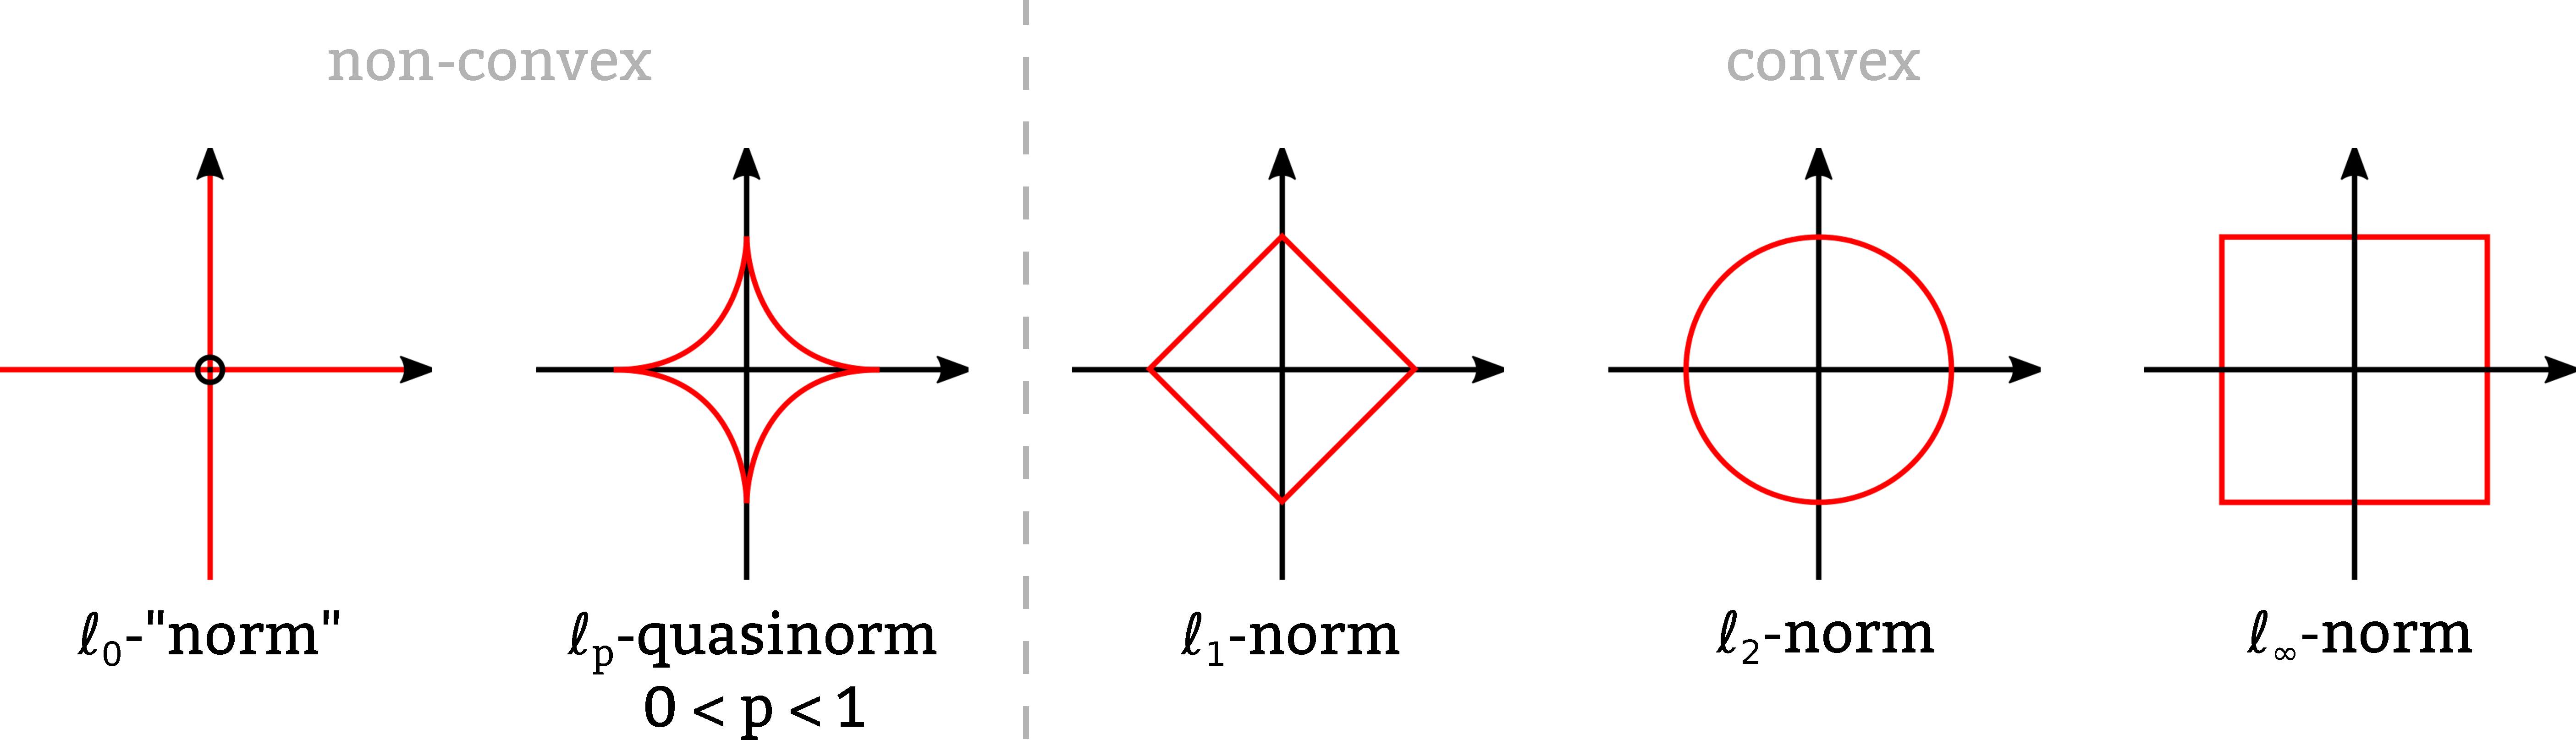
\includegraphics[width=\textwidth]{images/balls.pdf}
    \caption{\textbf{$\ell_p$ balls in 2D.}}
    \label{fig:balls}
\end{figure}

\begin{notation}
$[n]$ denotes the set of integers form $0$ to $n-1$.
\end{notation}

\begin{remark}
Using the schema above, it is impossible to have a proper norm for $p = 0$; nonetheless, is very common to define $\ell_0$-norm as the number of non-zero coordinates:
\[\norm{\mathbf{x}}_0 = \left| \left\{x_i \ne 0 : i \in [n]\right\}\right| \text{ where } \mathbf{x} \in \mathbb{C}^N.\]
Following this convention, $\norm{\cdot}_0$ always refers to that formulation in this work.
\end{remark}

\begin{definition}
The Frobenius norm on $\mathbb{C}^{m \times n}$ is defined as
\[\norm{\mathbf{A}}_F = \left(\sum_{i=1}^m\sum{j=1}{n}|a_{ij}|^2\right)^\frac{1}{2}.\]
\end{definition}

\begin{definition}[sparsity]
We call a vector $s$-sparse, if at most $s$ of its entries are non-zero; i.e. $\norm{\mathbf{x}}_0 \le s$.
\end{definition}

\begin{notation}
By $\Sigma_s^N$ we denote the set of all s-sparse vectors in $\mathbb{C}^N$; that is,
\[\Sigma_s^N = \left\{\mathbf{x} \in \mathbb{C}^N : \norm{\mathbf{x}}_0 \le s \right\}.\]
\end{notation}

%\begin{notation}
%The solution set $\left\{\mathbf{x} \in \mathbb{C}^N : \mathbf{Ax} = \mathbf{y}\right\}$ is denoted by $L_\mathbf{A}(\mathbf{y})$ for a given $\mathbf{A} \in \mathbb{C}^{m \times N}$.
%\end{notation}

%\begin{definition}[unique sparse solution]
%A vector $\mathbf{x}_* \in \mathbb{C}^N$ is the unique $s$-sparse solution of equation $\mathbf{Ax} = \mathbf{y}$ with $\mathbf{A} \in \mathbb{C}^{m \times N}$ and $\mathbf{y} \in \mathbb{C}^m$, if $L_\mathbf{A}(\mathbf{y}) \cap \Sigma_s^N = \{\mathbf{x}_*\}$, in other words, it is the only $s$-sparse vector satisfying the  linear system defined by $\mathbf{A}$ and $\mathbf{y}$.
%\end{definition}

\begin{definition}[kernel/null space]
The kernel/null space of a matrix $\mathbf{A} \in \mathbb{C}^{m \times N}$ is defined as
\[ker(\mathbf{A}) = \left\{\mathbf{x} \in \mathbb{C}^N : \mathbf{Ax} = \mathbf{0}\right\}.\]
\end{definition}

\begin{definition}[convex functions]
A function $f:\mathbb{C}^n \rightarrow \mathbb{R}$ is called convex, if for all $\mathbf{x}, \mathbf{y} \in \mathbb{C}^n $ and $t\in [0,1]$
\[f(t\mathbf{x} + (1-t)\mathbf{y}) \le t f(\mathbf{x}) + (1-t) f(\mathbf{y})\]
holds. Similarly, a function $f:\mathbb{C}^n  \rightarrow \mathbb{R}$ is called \textbf{strictly} convex, if for all $\mathbf{x} \ne \mathbf{y} \in \mathbb{C}^n $ and $t\in [0,1]$
\[f(t\mathbf{x} + (1-t)\mathbf{y}) < t f(\mathbf{x}) + (1-t) f(\mathbf{y})\]
holds.
\end{definition}

\begin{remark}
For $1 \le p < \infty$, the $\ell_p$-norms are strictly convex, and $\ell_p$-quasinorms for $0 < p < 1$ are always non-convex (see fig.~\ref{fig:balls}).
\end{remark}

\begin{remark}
A useful property of convex function is that all local minimizers are also global minimizers. Moreover, the minimizer of a \textit{strictly} convex function is unique, as well.
\end{remark}

\begin{definition}[Lipschitz-continuity]
A function $f:\mathbb{C}^n \rightarrow \mathbb{R}$ is said to be Lipschitz-continuous, if there exists a constant $L \in \mathbb{R}$ such that for all $\mathbf{x}, \mathbf{y} \in \mathbb{C}^n$
\[|f(\mathbf{x}) - f(\mathbf{y})| \le L \norm{\mathbf{x} - \mathbf{y}}_2\]
holds where $L$ is referred to as Lipschitz-constant.
\end{definition}

\begin{remark}
The set of Lipschitz-continuous functions is a superset of continuously differentiable functions.
\end{remark}

\begin{definition}[gradient and Hessian]
The gradient $\nabla f$ and the Hessian $\mathbf{H}_f$ of a function $f:\mathbb{C}^n \rightarrow \mathbb{R}$ at $\mathbf{x} \in \mathbb{C}^n$ is defined as follows:
\[\nabla f(\mathbf{x}) = \begin{bmatrix}
\frac{\partial}{\partial x_1} f(\mathbf{x}) \\ 
\frac{\partial}{\partial x_2} f(\mathbf{x}) \\ 
\vdots \\ 
\frac{\partial}{\partial x_n} f(\mathbf{x})
\end{bmatrix}, \mathbf{H}_f(\mathbf{x}) = \begin{bmatrix}
\frac{\partial^2}{\partial x_1^2} f(\mathbf{x}) & \frac{\partial^2}{\partial x_1 x_2} f(\mathbf{x}) & \ldots & \frac{\partial^2}{\partial x_1 x_n} f(\mathbf{x}) \\ 
\frac{\partial^2}{\partial x_2 x_1} f(\mathbf{x}) & \frac{\partial^2}{\partial x_2^2} f(\mathbf{x}) & \ldots & \frac{\partial^2}{\partial x_2 x_n} f(\mathbf{x}) \\ 
\vdots & \vdots & \ddots & \vdots \\ 
\frac{\partial^2}{\partial x_n x_1} f(\mathbf{x}) & \frac{\partial^2}{\partial x_n x_2} f(\mathbf{x}) & \ldots & \frac{\partial^2}{\partial x_n^n} f(\mathbf{x})
\end{bmatrix}.\]
\end{definition}

\begin{remark}
The geometric interpretation of gradient is that it is a vector in the tangent plane at a certain point on the surface defined by the function $f$, and this vector steepest direction where the value of $f$ increases the quickest. The Hessian, on the other hand, carries information about the curvature of the surface.
\end{remark}

\begin{definition}[order and rate of convergence]
An iterative method producing the sequence $\{\mathbf{x}_n\}$ is said to have a convergence of order $p$ to some $\mathbf{x}^*$ with respect to function $f:\mathbb{C}^n \rightarrow \mathbb{R}$, if there exists a number $\mu \in \mathbb{R}_+  \cup \{0\}$, called rate of convergence, such that
\[\lim_{k \rightarrow \infty} \frac{\norm{\mathbf{x}_{k+1} - \mathbf{x}^*}}{\norm{\mathbf{x}_{k} - \mathbf{x}^*}^p} < \mu.\]
\end{definition}

\begin{remark}
If $p = 1$, then the convergence is also referred to as a linear convergence. The special cases of linear convergence are \textit{superlinear} convergence when $\mu = 0$ and \textit{sublinear} convergence when $\mu > 0$. If $p=2$, then the convergence is called \textit{quadratic}.
\end{remark}

\begin{notation}
Besides the definition above, there are two other commonly used formulation to characterize the convergence speed using the big O notation. One way is expressing the time complexity by number of steps needed to approximate the solution under the maximal tolerated error $\epsilon$. For example, $ \mathcal{O}(\epsilon^-2)$ is a colloquial notation to express that the function will produce the approximation $\mathbf{x}_k$ such that 
\[|f(\mathbf{x}_{k}) - f(\mathbf{x}^*)| < \epsilon\]
after at most $k = \frac{1}{\epsilon^2}$ steps. The other way around is expressing the error in cost function by the number the already performed steps. Namely, $\mathcal{O}(k^\frac{1}{p})$ convergence states that
\[|f(\mathbf{x}_k) - f(\mathbf{x}_*)| < \frac{C\norm{\mathbf{x}_{0} - \mathbf{x}^*}_2^2}{k^\frac{1}{p}}\]
for some $C \in \mathbb{R}$.
\end{notation}

\begin{remark}
Note that using this notation, $\mathcal{O}(\epsilon^{-p})$ corresponds to $\mathcal{O}(k^{-\frac{1}{p}})$ (where $p$ has the same meaning as in the definition above), and that $\mathcal{O}(\epsilon^\alpha)$ means faster convergence than $\mathcal{O}(\epsilon^\beta)$, if $\alpha < \beta$.
\end{remark}

\begin{definition}[discrete Fourier transform (DFT)]
The discrete Fourier transform $\mathbf{\hat{x}} \in \mathbb{C}^m$ of a vector $\mathbf{x} \in \mathbb{C}^m$ is given by
\[\hat{x}_k = \sum_{l = 0}^{m-1} x_l \cdot e^{-\frac{2\pi i}{m}kl} : 0 \le k \le m-1,\]
or in matrix notation
\[\mathbf{\hat{x}} = \mathbf{Fx} \text{ with } F_{k,l} = e^{-\frac{2\pi i}{m}kl}.\]
\end{definition}

\begin{definition}[matrix rank]
The column rank of a matrix $\mathbf{A} \in \mathbb{C}^{m \times N}$ is defined as the maximal number of independent columns of $A$. Similarly, the row rank of a matrix $\mathbf{A} \in \mathbb{C}^{m \times N}$ is the maximal number of independent rows. As the column rank and the row rank are always equal, this number is simply called the rank of $A$.
\end{definition}

\begin{theorem}[SVD]
For $\mathbf{A} \in \mathbb{C}^{m \times N}$, there exist unitary matrices $\mathbf{U} \in \mathbb{C}^{m \times m}$, $\mathbf{V} \in \mathbb{C}^{N \times N}$, and uniquely defined non-negative numbers $\sigma_1 \ge \sigma_2 \ge \ldots \ge \sigma_{min\{m,N\}} \ge 0$ called singular values of $\mathbf{A}$, such that 
\[\mathbf{A} = \mathbf{U \Sigma V^*} \text{ where } \mathbf{\Sigma} = diag[\sigma_1, \sigma_2, \ldots, \sigma_{min\{m,N\}}] \in \mathbb{R}^{m \times N}.\]
The process of obtaining these matrices is called Singular Value Decomposition (SVD).
\end{theorem}

\begin{remark}
SVD is a particularly useful in analysis of matrix rank as the rank of a matrix always coincides with the number of its non-zero sigular values.
\end{remark}

\end{tight_equations}

\section{Basics of Compressed Sensing}
As it was shortly mentioned in chapter~\ref{chapter:introduction}, a mathematical framework called compressed sensing (CS) revolutionized MR image acquisition process allowing reconstruction from much fewer k-space values \textit{under certain conditions} as it would be necessary according to the Nyquist criterion.

To realize this promise, first and foremost, the signal to be recovered must be sparse in some transform domain. Fortunately, natural images are intrinsically sparse in the Fourier domain and in many other wavelet domains, MR images are being no exception to that, and as MRI scanners operates on Fourier transform, the sparsity condition is always satisfied by the very nature of the imaging process. The other conditions, however, are less intuitive, hence in this section we attempt to give a quick overview of the most important definitions and theorems needed for basic understanding.

\subsection{Formulation of the Problem}\label{section:problem formulation}
In engineering settings, especially in signal processing context, engineers and scientist usually try first to model physical systems by a linear model because that way they describe the problem by a set of linear expressions, and then they can express it as a matrix-vector multiplication $\mathbf{Ax} = \mathbf{y}$, where vector $\mathbf{x}$ is the input of the system, vector $\mathbf{y}$ is the output (measured data), and $\mathbf{A}$ characterizes the measurement (thus it is often referred to as \textit{measurement matrix}). A very common task then is to recover the input consisting of $N$ variables from the measurement data, and generally the number of measurements $m$ must obey $m > N$, otherwise the linear system is underdetermined, and hence there exist infinitely many solutions. In case of MRI setting, this statement corresponds to already mentioned Nyquist criterion that requires the sampling frequency in k-space to be twice as the highest frequency in the image space (vid. $k_{FOV} = 2 \cdot k_{max}$ in section~\ref{section:accelerated}).

And that is the point when compressed sensing comes into play claiming that given a \textit{proper} measurement matrix $\mathbf{A}$, the problem

\begin{equation}
    \tag{P\textsubscript{0}}\label{eq:P_0}
    \min_{\mathbf{z} \in \mathbb{C}^N} \norm{\mathbf{z}}_0 \text{ subject to } \mathbf{Az} = \mathbf{y} = \mathbf{Ax}
\end{equation}
have a unique $s$-sparse solution with $s \ll N$. This optimization problem is often referred to as (\ref{eq:P_0}). The number of necessary measurement, however, still a difficult question. There are theoretical results stating that $m = 2s$ is the lower bound for a perfect recovery~\citationneeded and that a stable recovery (later explained) occurs with high probability with $m \ge C s log(N / m)$ for random measurement matrices~\citationneeded, but in practice, reconstruction algorithms struggle to reach these theoretical limits (albeit, the achieved $m$ is still drastically improved compared to the Nyquist sampled case).

The main reason why the optimal bounds are usually not reached is that the measurement matrices of real life systems have often have less favorable properties as random matrices and, more importantly, (\ref{eq:P_0}) is a NP-hard problem~\citationneeded; thus, only relaxations can be solved. The most commonly used relaxations are the so called $\ell_1$ minimization or Basis Pursuit (BP)~\citationneeded defined as
\begin{equation}
    \tag{P\textsubscript{1}}\label{eq:P_1}
    \min_{\mathbf{z} \in \mathbb{C}^N} \norm{\mathbf{z}}_1 \text{ subject to } \mathbf{Az} = \mathbf{y},
\end{equation}
the Basis Pursuit DeNoising (BPDN)~\citationneeded formulated as

\begin{equation}
    \tag{P\textsubscript{1}, \texteta}\label{eq:P_1_noisy}
    \min_{\mathbf{z} \in \mathbb{C}^N} \norm{\mathbf{z}}_1 \text{ subject to } \norm{\mathbf{Az} - \mathbf{y}}_2 \le \eta,
\end{equation}
and the LASSO (Least Absolute Shrinkage and Selection Operator)~\citationneeded problem expressed by
\[\min_{\mathbf{z} \in \mathbb{C}^N} \norm{\mathbf{Az} - \mathbf{y}}_2 \text{ subject to } \norm{\mathbf{z}}_1 \le s.\]
By the aid of a Lagrangian multiplier $\lambda$, the latter two can be transformed to the same unconstrained minimization problem
\[\min_{\mathbf{z} \in \mathbb{C}^N} \norm{\mathbf{Az} - \mathbf{y}}_2 + \lambda \norm{\mathbf{z}}_1.\]

\subsection{Conditions and Guarantees}
While $\ell_1$-relaxation (often referred to as (\ref{eq:P_1}) problem) might be appealing as it can be solved efficiently in polynomial time, it needs a more careful approach to guarantee that the minimum of the $\ell_1$ problem is also a solution of (\ref{eq:P_0}). The $\ell_2$-relaxation, for example, always has a unique solution, but this solution is not necessarily sparse (for a figurative illustration, see fig.~\ref{fig:sparse_solution} and fig.~\ref{fig:3D_l1_min}). In contrast, $\ell_1$ problem has a solution which is both unique and $s$-sparse given that the matrix $\mathbf{A}$ fulfills the so called \textit{null space property} of order $s$, introduced by Cohen, Dahmen and DeVore in~\cite{cohen_compressed_2009}.

\begin{figure}[tb]
    \centering
    \begin{minipage}{.63\textwidth}
        \centering
        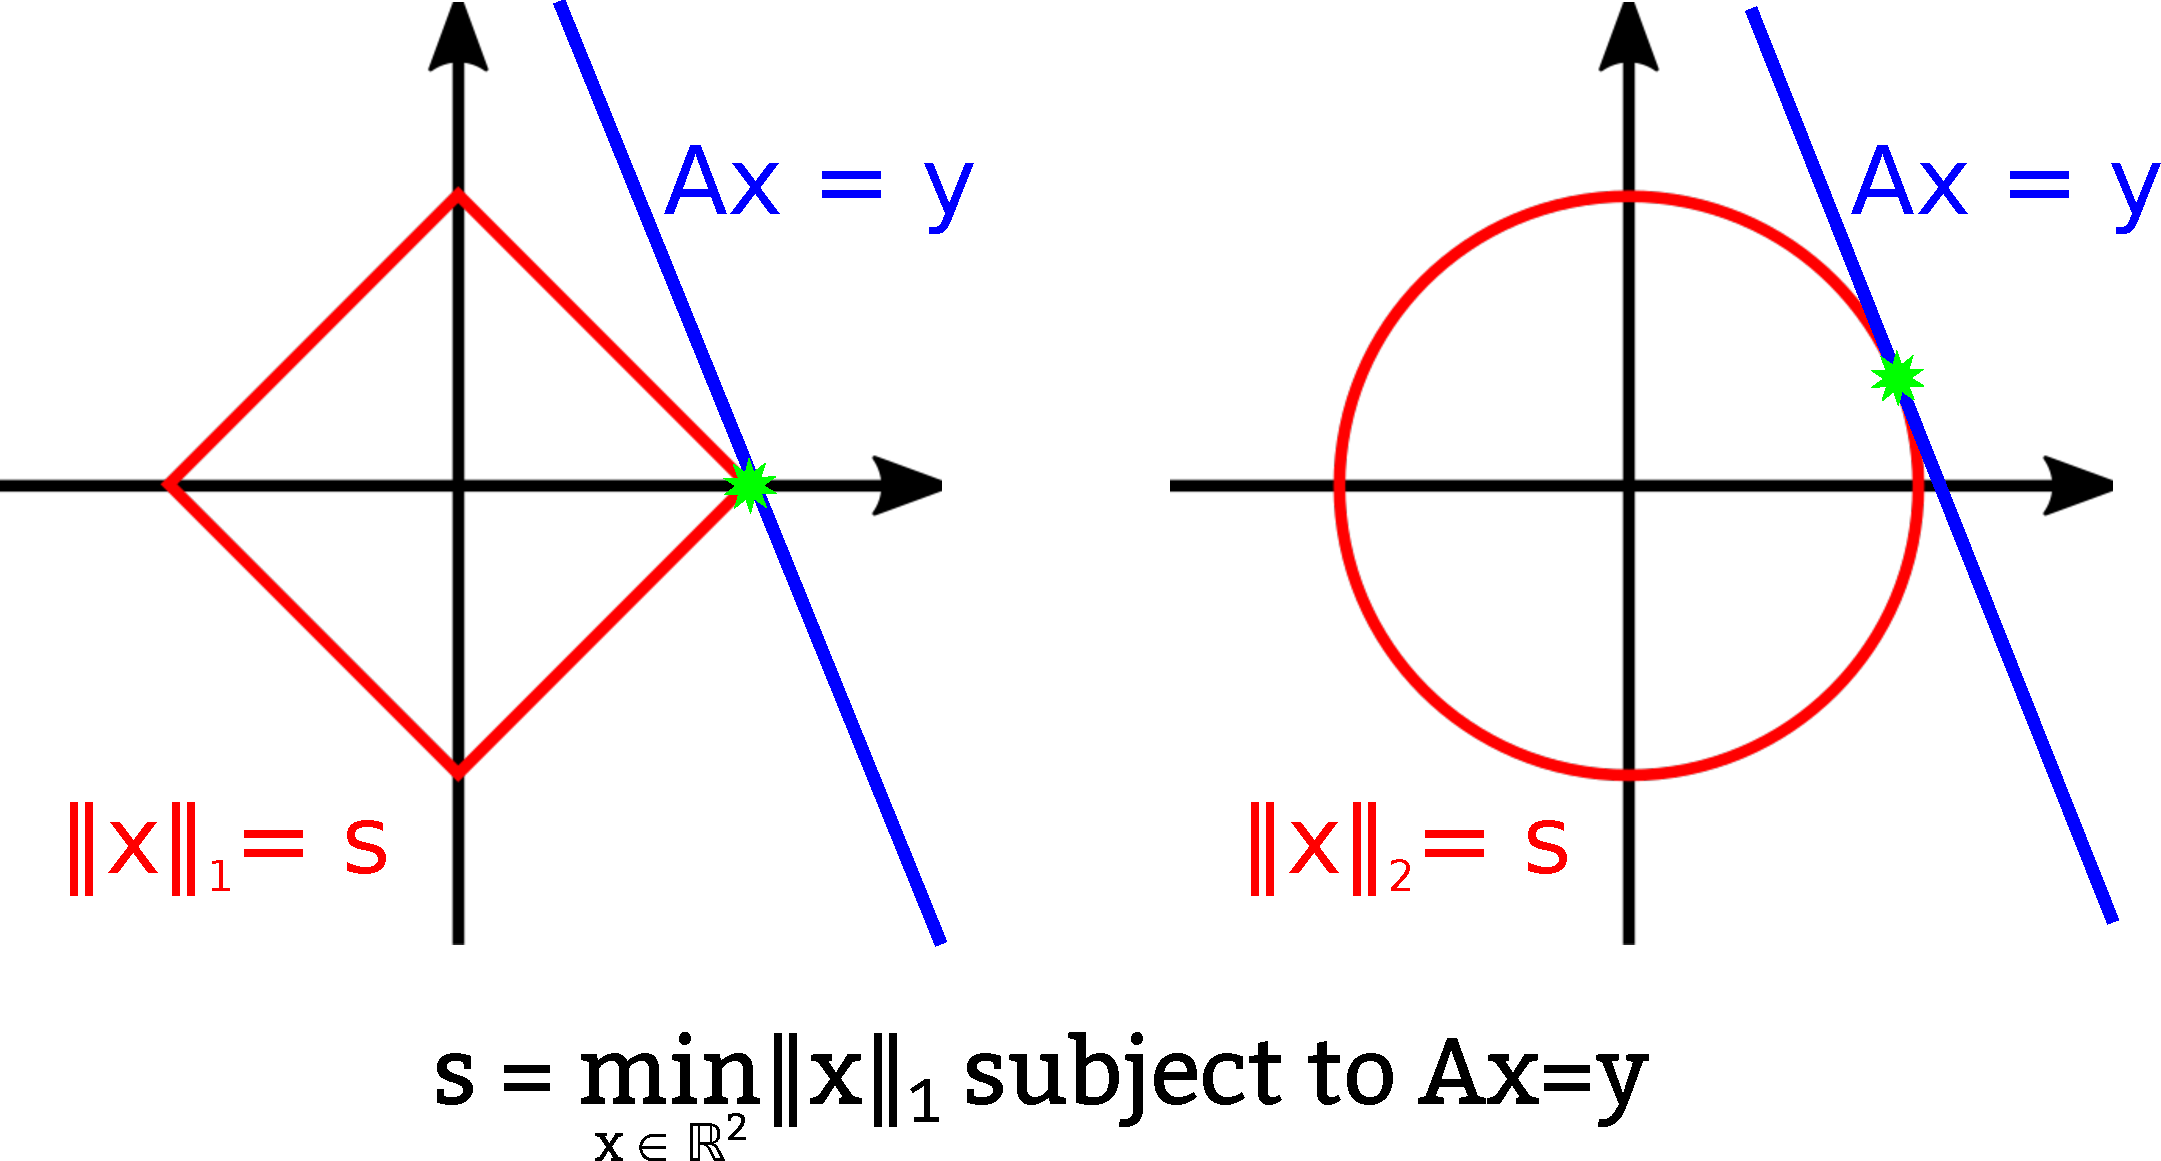
\includegraphics[width=0.7\linewidth]{images/sparse_solution.pdf}
        \caption{\textbf{Solution of $\ell_1$ and $\ell_2$ minimization problems.} Matrix $\mathbf{A} \in \mathbb{R}^{1 \times 2}$ is an underdetermined linear system, and the task is to find $\mathbf{x} \in \mathbb{R}^2$ with minimal $\ell_1$-norm such that it satisfies the equation $\mathbf{Ax} = \mathbf{y}$ for fixed $\mathbf{y} \in \mathbb{R}$. The number of solutions are infinite (all points along the blue line), and the unique solution of minimization problem is marked with a green star. Note that $\ell_1$ minimization gives sparse solution, while $\ell_2$ minimization is not sparsity seeking.}
        \label{fig:sparse_solution}
    \end{minipage}%
    \hspace{0.02\textwidth}
    \begin{minipage}{0.34\textwidth}
        \centering
        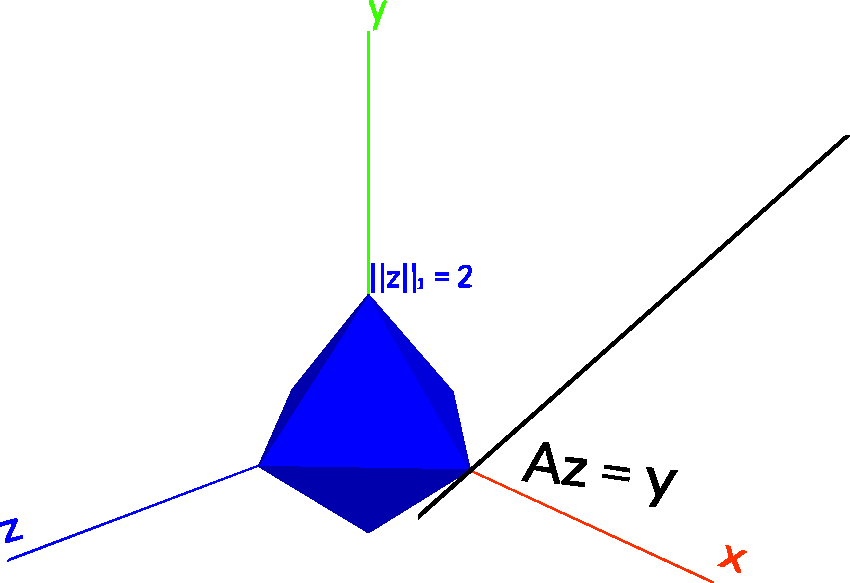
\includegraphics[width=\linewidth]{images/3D_l1_min.pdf}
        \caption{\textbf{$\ell_1$ minimization in 3D.} This figure demonstrates the sparsity seeking nature of $\ell_1$ minimization in a 3-dimensional space. The image is taken from the interactive demo available at \url{https://hakkelt.github.io/CS-demo/}}
        \label{fig:3D_l1_min}
    \end{minipage}
\end{figure}

\begin{definition}[NSP]
A matrix $\mathbf{A} \in \mathbb{C}^{m \times N}$ is said to satisfy the null space property (NSP) of order $s$, if for any set $S \subset [N]$ with $|S| = s$
\[\norm{\mathbf{v}_S}_1 < \norm{\mathbf{v}_{S^C}}_1 : \forall \mathbf{v} \in ker(\mathbf{A})  \setminus \{\mathbf{0}\}.\]
\end{definition}

\begin{notation}
For a vector $\mathbf{v} \in \mathbb{C}^N$ and a set $S \subset [N]$, we denote by $\mathbf{v}_S$ either the vector in $\mathbb{C}^{|S|}$ which is the restriction of $\mathbf{v}$ to the indices in $S$, or the vector in $\mathbb{C}^N$ which coincides with $\mathbf{v}$ on the indices in $S$ and is zero elsewhere. Similarly, $\mathbf{v}_{S^C}$ means the same with the complement of $S$.
\end{notation}

\begin{theorem}
Given a matrix $\mathbf{A} \in \mathbb{C}^{m \times N}$, every $s$-sparse vector $\mathbf{x} \in \Sigma_s^N \subset \mathbb{C}^N$ is the unique solution of (\ref{eq:P_1}) with $\mathbf{y} = \mathbf{Ax}$ if and only if $\mathbf{A}$ satisfies the NSP of order $s$.
\end{theorem}

\begin{remark}
This theorem shows that for every $\mathbf{y} = \mathbf{Ax}$ with $s$-sparse $\mathbf{x}$, the $\ell_1$-minimization (\ref{eq:P_1}) actually solves the $\ell_0$-minimization (\ref{eq:P_0}) when the NSP of order $s$ holds.
\end{remark}

Although NSP is a formidable construct that allows relatively easy and straightforward proofs, in realistic settings, signals are rarely sparse, but rather \textit{almost} $s$-sparse vectors, meaning that the most part of the energy of the signal is concentrated in $s$ coefficients with the the largest values. To involve these cases in the compressed sensing framework, an extension of NSP is used, called \textit{stable NSP}. Proving the stable NSP property, one can then approximate the almost $s$-sparse signal with the \textit{best $s$-term approximation} having a tight bound on the error term.

\begin{definition}[$\ell_p$-error of best $s$-term approximation]
For $p > 0$, the $\ell_p$-error of best $s$-term approximation to a vector $\mathbf{x} \in \mathbb{C}^N$ is defined by
\[\sigma_s(\mathbf{x})_p = \inf\left\{\norm{\mathbf{x} - \mathbf{z}}_p : \mathbf{z} \in \Sigma_s^N\right\}.\]
\end{definition}

\begin{remark}
The  infimum is always achieved by an $\mathbf{z} \in \Sigma_s^N$ whose non-zero entries equal the $s$ largest absolute entries of $\mathbf{x}$.
\end{remark}

\begin{definition}[stable NSP]
A matrix $\mathbf{A} \in \mathbb{C}^{m \times N}$ is said to satisfy the stable NSP with constant $0 < \rho < 1$ of order $s$, if for any set $S \subset [N]$ with $|S| = s$
\[\norm{\mathbf{v}_S}_1 \le \rho \norm{\mathbf{v}_{S^C}}_1 : \forall \mathbf{v} \in ker(\mathbf{A}).\]
\end{definition}

\begin{theorem}
The matrix $\mathbf{A} \in \mathbb{C}^{m \times N}$ satisfies the stable NSP with constant $0 < \rho < 1$ of order $s$ if and only if for any set $S \subset [N]$ with $|S| = s$
\begin{equation}\label{eq:stable_nsp}
    \norm{\mathbf{z} - \mathbf{x}}_1 \le \frac{1 + \rho}{1 - \rho} \left(\norm{\mathbf{z}}_1 - \norm{\mathbf{x}}_1 + 2\norm{\mathbf{x}_{S^C}}\right)
\end{equation}
holds for any set $S \subset [N]$ with $|S| = s$ and for all vectors $\mathbf{x,z} \in \mathbb{C}^N$ with $\mathbf{Az} = \mathbf{Ax}$.
\end{theorem}

\begin{remark}
The estimation (\ref{eq:stable_nsp}) can be upper-bounded by means of the $\ell_1$-error of best $s$-term approximation $\sigma_s(\mathbf{x})_1$ as
\[\norm{\mathbf{z} - \mathbf{x}}_1 \le \frac{1 + \rho}{1 - \rho} \left(\norm{\mathbf{z}}_1 - \norm{\mathbf{x}}_1 + 2\norm{\mathbf{x}_{S^C}}\right) \le 2 \cdot \frac{1 + \rho}{1 - \rho}\sigma_s(\mathbf{x})_1.\]
\end{remark}

The significance of this theorem is that it implies that having the stable NSP fulfilled, the unique $s$-sparse solution $\mathbf{z}$ of (\ref{eq:P_1}) with $\mathbf{y} = \mathbf{Ax}$ approximates the vector $\mathbf{x}$ with a bounded $\ell_1$-error. Therefore, by a good approximation of the sparsity $s$ of the signal and an upper bound $\epsilon$ of $\sigma_s(\mathbf{x})_1$ (both can be inferred by the statistics of the signal), one can construct or select a measurement matrix $\mathbf{A}$ such that the solution of \textit{any} algorithm solving (\ref{eq:P_1}) is an approximation of the input signal with the maximal error of
\[\frac{1 + \rho}{1 - \rho} \cdot 2\epsilon,\]
where $\rho$ depends only on the measurement matrix and $\epsilon$ is a small number because only little energy is stored in the entries contributing the the $\ell_p$-error of best $s$-term approximation.
Practically that means that by the careful design of the measurement, arbitrary precision recovery is possible (having Nyquist sampling as a special case for guaranteed perfect recovery), and that in case of approximately $s$-sparse signals, the number of measurements can be drastically reduced without significant amount of error introduced.

Finally, this construct can be further extended  to handle noisy measurement: proving the \textit{robust NSP} for the measurement matrix, the same guaranties apply to the $\ell_1$-error as in case of stable recovery, extended by an extra term characterizing the noise on the measurement. As a result, arbitrary precision is allowed for arbitrary optimization algorithm capable of solving (\ref{eq:P_1_noisy}) given a measurement matrix satisfying the \textit{robust NSP}.

\begin{definition}[robust NSP]
A matrix $\mathbf{A} \in \mathbb{C}^{m \times N}$ is said to satisfy the robust NSP with constants $0 < \rho < 1$ and $0 < \tau$ of order $s$, if for any set $S \subset [N]$ with $|S| = s$
\[\norm{\mathbf{v}_S}_1 \le \rho \norm{\mathbf{v}_{S^C}}_1 + \tau \norm{\mathbf{Av}}_2 : \forall \mathbf{v} \in \mathbb{C}^N.\]
\end{definition}

\begin{remark}
Note that $\mathbf{v}$ is not required to be in $ker(\mathbf{A})$.  In fact, if $\mathbf{v} \in ker(\mathbf{A})$, then $\mathbf{Av} = \mathbf{0}$, and we obtain the definition of stable NSP. Therefore, the robust NSP implies stable NSP.
\end{remark}

\begin{theorem}
The matrix $\mathbf{A} \in \mathbb{C}^{m \times N}$ satisfies the robust NSP with constants $0 < \rho < 1$ and $0 < \tau$ of order $s$ if and only if
\begin{equation}\label{eq:robust_nsp}
    \norm{\mathbf{z} - \mathbf{x}}_1 \le \frac{1 + \rho}{1 - \rho} \left(\norm{\mathbf{z}}_1 - \norm{\mathbf{x}}_1 + 2\norm{\mathbf{x}_{S^C}}\right) + \frac{2\tau}{1-\rho}\norm{\mathbf{A(z-x)}}_2
\end{equation}
holds for any set $S \subset [N]$ with $|S| = s$ and for all vectors $\mathbf{x,z} \in \mathbb{C}^N$ with $\mathbf{Az} = \mathbf{Ax}$.
\end{theorem}

\begin{remark}
Supposing that a matrix $\mathbf{A} \in \mathbb{C}^{m \times N}$ satisfies the robust NSP of order $s$, (\ref{eq:robust_nsp}) implies that for any $\mathbf{x} \in \mathbb{C}^N$, a solution $\mathbf{z}$ of (\ref{eq:P_1_noisy}) with $\norm{\mathbf{Ax - y}} \le \eta$ approximates $\mathbf{x}$ with $\ell_1$-error \footnote{Number $4$ in the numerator of the error term at (\ref{eq:error_bound}) is not a typo as one would expect, but a counterintuitive result of some basic arithmetics leading to this expression.}
\begin{equation}\label{eq:error_bound}
    \norm{\mathbf{z} - \mathbf{x}}_1 \le 2 \cdot \frac{1 + \rho}{1 - \rho}\sigma_s(\mathbf{x})_1 + \frac{4\tau}{1-\rho}\eta.
\end{equation}
\end{remark}

The main problem, nevertheless, with the NSP is that proving it is actually NP-hard in general. Hence, the \textit{restricted isometry property (RIP)} is more commonly used in theoretical works because it is easier to handle, and at the same time it implies stable NSP.

\begin{definition}[RIP]
A matrix $\mathbf{A} \in \mathbb{C}^{m \times N}$ is said to satisfy the $s$-restricted isometry property with the smallest number $0 < \delta_s < 1$, called restricted isometry constant (RIC), if
\[(1 - \delta_s)\norm{\mathbf{x}}_2^2 \le \norm{\mathbf{Ax}}_2^2 \le (1 + \delta_s)\norm{\mathbf{x}}_2^2\]
holds for add $\mathbf{x} \in \Sigma_s^N$.
\end{definition}

\begin{theorem}
If a matrix $\mathbf{A} \in \mathbb{C}^{m \times N}$ has restricted isometry constant 
\[\delta_{2s} < \frac{1}{\sqrt{2}},\] then it satisfies the robust NSP of order $s$ with constants
\[\rho = \frac{\delta_{2s}}{\sqrt{1 - \delta_{2s}^2}} \text{ and } \tau = \frac{2\sqrt{s}}{(1-\delta_{2s}\sqrt{1 + \delta_{2s}}}.\]
\end{theorem}

\subsection{The Connection Between CS and MRI}
Although it is not always trivial to apply the compressed sensing scheme to different measurement methods, MR imaging is in a lucky position with the Fourier transform in the core of its image acquisition process as random partial discrete Fourier transform (i.e., selecting $m$ rows randomly with uniform distribution from the $N$ rows, or in other words, observing only $m$ entries of the Fourier transform) is proved to satisfy the RIP~\cite{fornasier_theoretical_2010}. That discovery has enormous significance as is offers a way to speed up the inherently slow MRI measurements by measuring only a few randomly selected points from the k-space, and then solve the $\ell_1$-minimization problem via an arbitrarily selected optimization algorithm.

\begin{figure}[htbp]
    \centering
    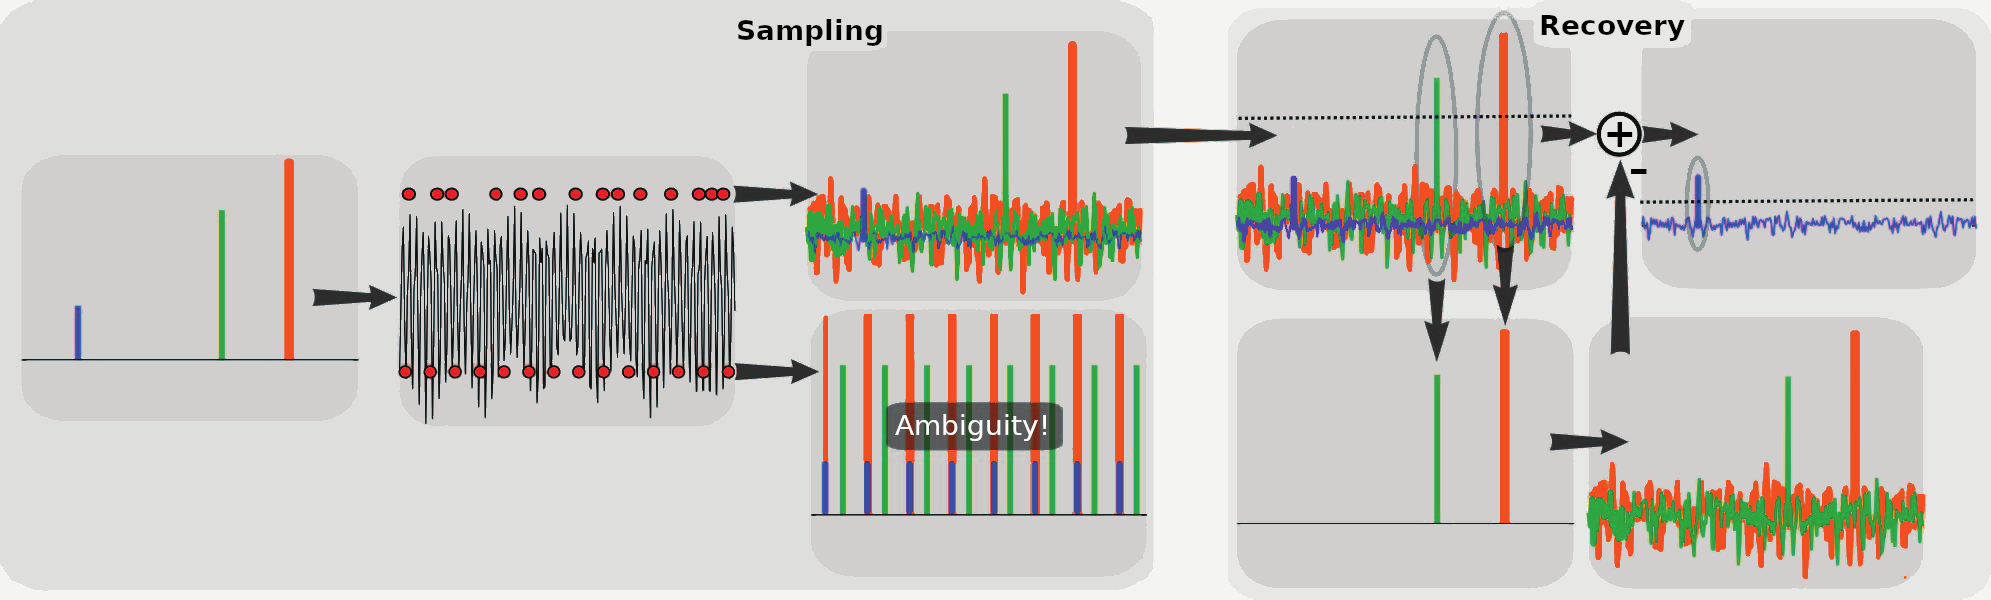
\includegraphics[width=0.9\linewidth]{images/random_sampling.png}
    \caption{\textbf{A heuristic reconstructing signal from random undersampling.} In the left block, the result of Fourier analysis is shown for both equidistant and random sampling, demonstrating the underdetermined nature of equidistant undersampling (bottom) and the noise-like effect of random sampling (top). In the right block, a simple method is applied that selects the peaks above a certain threshold as candidates, calculates the inference of these peaks, and substracts the calculated inference from the spectrum allowing detection of further peaks after lowering the threshold. Source: Adapted from~\cite{lustig_compressed_2008}.}
    \label{fig:random_sampling_1D}
\end{figure}

\begin{figure}[htbp]
    \centering
    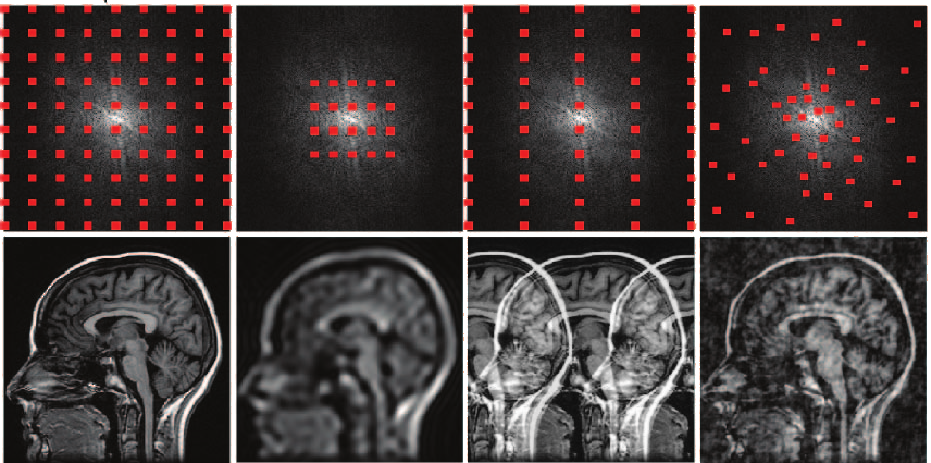
\includegraphics[width=0.8\linewidth]{images/random_sampling2.png}
    \caption{\textbf{Connection between the sampling pattern and the introduced inference.} Using inverse DFT replacing the missing values with zeros leads to different type of undersampling artifacts. Sampling only the center reduces the resolution, undersampled equispaced scheme adds shifted copies of the signal to the recovered image, and random sampling spreads the inference uniformly. Source: Adapted from~\cite{lustig_compressed_2008}.}
    \label{fig:random_sampling_images}
\end{figure}

One can think of this recovery scheme as a denoising or inference cancelling process where the noise/inference to be removed is the sum of undersampling artifacts predicted by Nyquist-Shannon theorem. If we use an equispaced sampling pattern, then the resulted noise is basically shifted copies of the signal and hence recovery of the original signal is impossible as each replica is an equally likely candidate. Figure~\ref{fig:random_sampling_1D} illustrates this problem and demonstrates the advantage of random sampling. In contrast, random sampling "spreads" the noise uniformly over the image, so the inference acts mostly like white noise (see fig.~\ref{fig:random_sampling_images}). This approach is particularly appealing as countless denoising algorithms exists, and as many of them are based on minimization of the $\ell_1$-norm of the transform of signal, these methods provide a convenient way to solve (\ref{eq:P_1}) problem. The transform used is always depends on the type of image in interest: MR angiograms (imaging technique visualizing blood vessels) are sparse even in the image domain, but edge detection algorithms like finite differences transform (that corresponds to the well-known total variation (TV) penalty) can further enhance sparsity (fig.~\ref{fig:MRA}); brain images have a sparse representation in various wavelet transformations~\ref{fig:brain_wavelet}, and dynamic MR images tend to be sparse after temporal Fourier transform is applied.

\begin{figure}[htbp]
    \centering
    \begin{minipage}[t]{0.65\linewidth}
        \centering
        \begin{tabular}{c}
            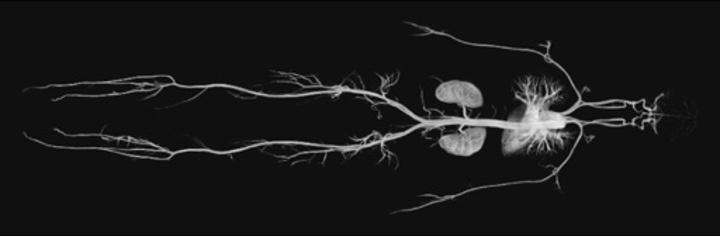
\includegraphics[width=0.95\linewidth]{images/MRI-Angiography.jpg}
            \\
            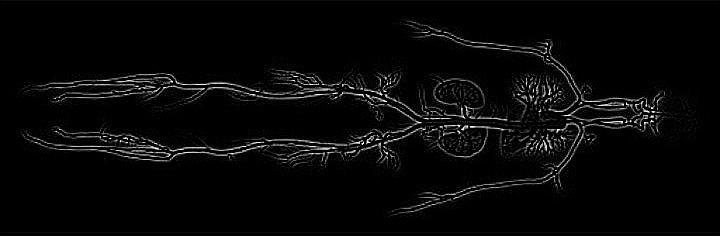
\includegraphics[width=0.95\linewidth]{images/MRI-Angiography_edges.jpg}
        \end{tabular}
        \caption{\textbf{MR angiograms} (MR images tuned to show blood vessels) are intrinsically sparse even in image domain (top image), but sparseness can be further improved by edge detection algorithms (botton image) because only the morphology of the blood vessels are diagnostically relevant. Source: Adapted from~\cite{noauthor_mri_nodate}.}
        \label{fig:MRA}
    \end{minipage}
    \hspace{0.02\linewidth}
    \begin{minipage}[t]{0.31\linewidth}
        \centering
        \begin{tabular}{c}
            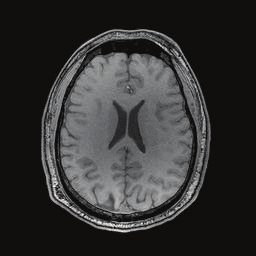
\includegraphics[width=0.65\linewidth]{images/brain_MRI.png}
            \\ 
            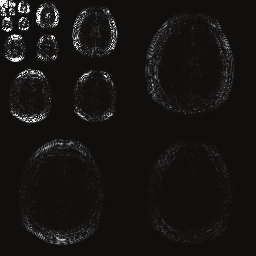
\includegraphics[width=0.65\linewidth]{images/brain_MRI_wavelet.png}
        \end{tabular}
        \caption{\textbf{MRI images of the brain} are not sparse in image domain, but they are in multiple wavelet transform domains. Source:~\cite{zhao_compressed_2014}.}
        \label{fig:brain_wavelet}
    \end{minipage}
\end{figure}

A truly random sampling in the k-space, however, is generally impractical due to hardware and physiological constraints. For example, the sampling must follow smooth lines and curves and be robust to real-life situations such as motion artifacts. Also, a uniform random distribution of samples in the spatial-frequency domain does not take into account the energy distribution of MR images in k-space. Therefore it makes more sense to opt for a nonuniform variable density sampling matching energy distribution in k-space. Precisely, we should consider having more samples from the central part of the frequency domain and less high frequency components. Consequently, carefully designed pseudo-random sampling trajectories are utilized in practice. To quantify  evaluate the "randomness" of the trajectories, authors of~\cite{lustig_compressed_2008} and~\cite{lustig_sparse_2007} suggested using point spread function (PSF) to measure the desirable incoherence of the aliasing interference, defined as
\[PSF = (\mathbf{e}_j^* \mathcal{F}_u^* \mathcal{F}_u \mathbf{e}_i)_{i,j}\]
where $\mathcal{F}_u$ is the undersampling Fourier transform operator, $\mathbf{e}_i$ and $\mathbf{e}_j$ are of the natural basis having $0$ in each coordinate except the $i$-th and $j$-th position, resprectively, where $1$ is located. Thus, $PSF_{i,j}$ measures the contribution of a unit-intensity pixel at the $i$-th position of the image to the $j$-th position in the k-space. In case of fully sampled measurement, the $PSF$ is an identity matrix, and undersampling induces non-zero off-diagonal terms. Figuratively speaking, $PSF$ measures the leakage of energy from a Kronecker delta input. Figure~\ref{fig:trajectory_coherence} shows $PSF$ for a central pixel for a couple sampling trajectories. This quantitiy then can serve as a simple measure for the incoherence by calculating the sidelobe-to-peak ratio:
\[SPR = \max_{i \ne j} \left|\frac{PSF_{i,j}}{PSF_{i,i}}\right|.\]
As a result, the design of an incoherent sampling trajetory aims to minimize $SPR$.

\begin{figure}
    \centering
    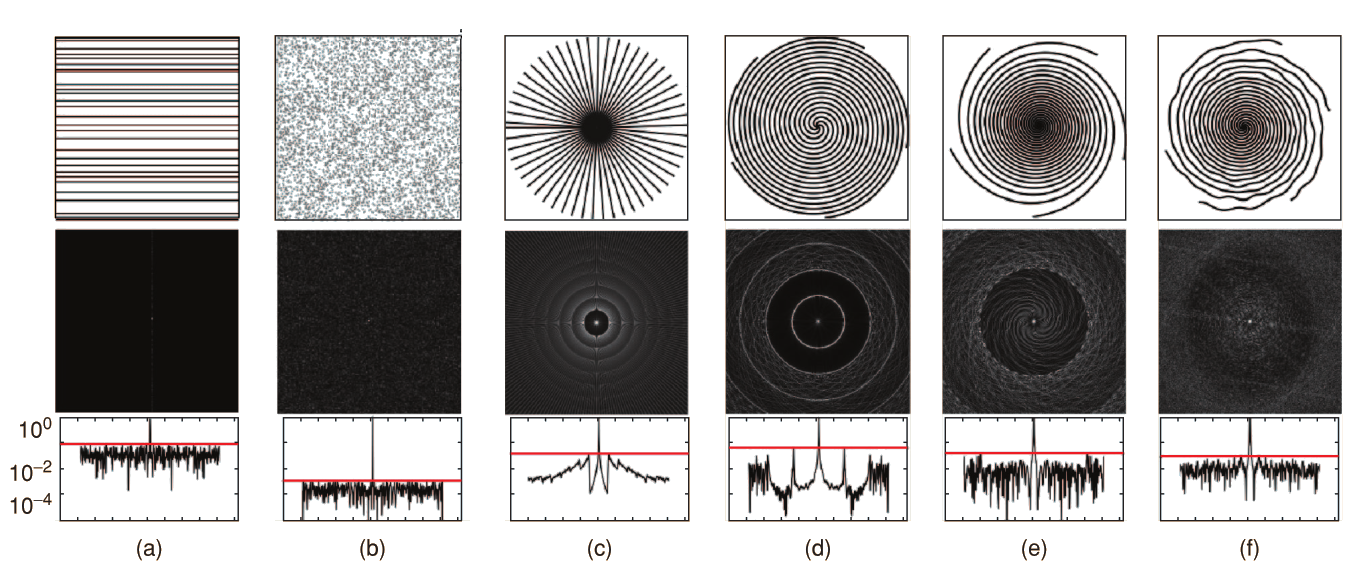
\includegraphics[width=0.98\linewidth]{images/PSF_trajectories.png}
    \caption{\textbf{$\mathbf{PSF}$ of the central pixel for various sampling trajectories:} (a) randomly chosen horizontal lines, (b) uniformly selected random points, (c) radial, (d) uniform spirals, (e) variable density spirals, and (f) variable density perturbed spirals. The red line marks the overall coherence level.\\
    Source: Adapted from~\cite{lustig_compressed_2008}.}
    \label{fig:trajectory_coherence}
\end{figure}

\section{Numerical Methods}

While the recovery is proved to be \textit{possible} via polynomial time algorithms minimizing the $\ell_1$-relaxation of ($\ref{eq:P_0}$), finding the best algorithm for a given use-case is a quite challenging problem as the algorithm must satisfy many constraints like fast convergence speed and guarantee for a (global) convergence, inexpensive computation and limited memory requirement, numerical robustness and lack of problem-dependent parameters. The number of choices are numberless; nevertheless, none of them appears to outperform all other in every aspects because improving convergence speed while keeping global convergence is difficult, increased computational speed usually comes at the cost of a more memory hungry implementation, and it is hard to optimize algorithms without tuning its parameters specifically to the problem to be solved.

The computation cost and the memory requirement, in particular, tend to be most restrictive constraint. Namely, the direct calculation of Hessian is often computationally prohibitive on one hand, on the other hand, the storage of the calculated Hessian can be problematic even for medium sized images. To see that, let us consider a $256 \times 256$ grayscale image. Storing all the $65536$ pixels of the image as a half-precision floating point number requires $256 \times 256 \times \SI{2}{\byte} = \SI{128}{\kibi\byte}$. While the gradient of the image is of the same size, the Hessian has a quadratic memory requirement, $(256 \times 256)^2 \times \SI{2}{\byte} = \SI{8}{\gibi\byte}$ in our example. Although this requirement can be satisfied even on a stronger personal computer, a high-resolution dynamic MR image, for instance, usually results in magnitudes larger allocations, like \SI{256}{\gibi\byte} for a 3D image of size $512\times512\times512$ with 512 time frames and an enormously large \SI{33554432}{\tebi\byte} allocation for its Hessian. 

Therefore, second order optimization algorithms (i.e., algorithms using second derivative) are not feasible in image reconstruction problems in general, even though these algorithms usually outperform first order methods in convergence speed. On the other end of the scale, zeroth order methods (that is, algorithms not using any gradient information), while being feasible and sometimes used for image reconstruction, are considered to be impractical due to their slow convergence. Therefore, first order methods appear to be the default option in nearly all image processing settings, and accordingly, we will discuss them exclusively in the following. Of course, even this restricted scope is far too large to cover, hence we restrict ourselves only to a few concepts that will serve as building blocks of more complex algorithms reviewed in the next chapters.

\subsection{General Gradient Descent}
Since Cauchy first proposed an iterative gradient direction method to solve astronomic calculations in 1847~\cite{cauchy_methode_1847}, the family of gradient descent algorithms became one of the largest and most popular group of solvers due to their simplicity and relatively inexpensive computation. The core of all gradient methods is the so called gradient step defined as
\[\mathbf{x}_{k+1} = \mathbf{x}_k + \alpha_k \nabla f(\mathbf{x_k}),\]
where $f$ is commonly called a loss or cost function, and $\alpha$ is generally referred to as step size and it is a negative number if we consider the minimization problem and positive if we are looking for the maximum.

The greatest advantage of gradient descent is that it is universally applicable to all problems where $f$ is differentiable, but it is capable to find only a local optimum, and, in its original form, it is rarely optimal (albeit sometimes the only feasible option). Additionally, finding the optimal step size and a proper starting point is quite challenging, and convergence is not always guaranteed. If the step size is too small then the convergence speed becomes impractically slow; on the other hand, too large step size can make the algorithm fail to converge. The improper choice of the initial point can also drastically delay convergence, and also might cause converge to a unfavorable local optimum instead of the global optimum (or, at least, a better optimum nearby).

\subsubsection{Selection of Step Size}
While a good starting point is always depends on the function to be minimized (from this point, we consider only the minimization problem without loss of generality), there are various schemes for determining the step size in each step. Notably, the line search methods are commonly used to solve this problem because of its universally applicability. As the name suggests, these methods perform a search for local minimum along a descent direction (which, in case of gradient methods, is given by the gradient) and return exactly the step size needed to step into this minimum. The search can be exact (like the later described conjugate gradient' implicit line search) or inexact where only an approximation of the local minimum is calculated (like backtracking line search~\cite{armijo_minimization_1966} (see also fig.~\ref{fig:backtracking}) or using Wolfe conditions~\cite{wolfe_convergence_1969}).

However, the line search methods become impractical when evaluation of the cost function is computationally expensive. In these cases only fixed (but not necessarily constant) step is applicable. Restricting the cost function to the set of convex and smooth (differentiable with $L$-Lipschitz-gradient) functions, the analysis of global convergence of first order methods with respect to step size selection becomes possible, still covering a very large part of practical problems. In the following, $f$ is always assumed to satisfy these conditions.

The simplest step size selection scheme is the constant step size, and if we choose the step size to be $\frac{1}{L}$ where $L$ is the Lipschitz constant of $\nabla f$, then monotonic descent is ensured and convergence to the global minimizer is guaranteed  as $f$ is assumed to be convex. The convergence rate of cost function is linear ($\mathcal{O}(1/k)$) as 
\[f(\mathbf{x}_k) - f(\mathbf{x}_*) \le \frac{L\norm{\mathbf{x}_0 - \mathbf{x}_*}}{4k + 2}\]
is proved to be a tight inaccuracy bound for the generated sequence~\cite{drori_performance_2014}. This rate, however, is undesirably slow, and therefore the optimal step size is a highly researched topic. Although it was only recently proved that the convergence rate of all first order method with constant step size is still linear at best~\cite{taylor_smooth_2017}, there is already a long history of accelerated gradient methods like conjugate gradient, heavy ball iterations, and fast gradient method.

\subsection{Conjugate Gradient Method}

To overcome the slow convergence rate of the classic gradient descent (GD) method, one can use a modified version of it, the conjugate gradient method (CG) developed by Hestenes and Stiefel~\cite{hestenes_methods_1952}, if the problem is defined by a symmetric (or self-adjoint in complex case) and positive-definite matrix. In that case, the direction of movement must be conjugate to the previous directions. Two non-zero vectors $\mathbf{u}$ and $\mathbf{v}$ are conjugate with respect to some $\mathbf{A}$ matrix, if \[\mathbf{u}^T\mathbf{Av} = \mathbf{0}.\]
Let us consider the following linear system as the subject of optimization:
\[\mathbf{Ax} = \mathbf{b},\]
where $\mathbf{A} $is symmetric, positive-definite and real matrix, and $\mathbf{b}$ is also known.

\subsubsection{As a direct method} Since $\mathbf{A}$ is symmetric and positive-definite, it defines an inner product:
\[\langle \mathbf{u}, \mathbf{v} \rangle_\mathbf{A} := \mathbf{u}^T\mathbf{Av}.\]
Using that inner product, it is possible to find $n$ pairwise conjugate vectors: $\mathcal{P} = \{\mathbf{p}_1,...\mathbf{p}_n\}$. Then $\mathcal{P}$ forms a basis in $\mathbb{R}^n$, so the solution ($\mathbf{x_*}$) of optimization problem can be represented in terms of that basis:
\begin{equation} \label{eq:direct_method}
    \mathbf{x_*} = \sum_{i=1}^{n} \alpha_i \mathbf{p}_i.
\end{equation}
Left multiplying both sides with $\mathbf{p}_k^T \mathbf{A}$ we get:
\[\mathbf{p}_k^T\mathbf{Ax_*} = \sum_{i=1}^{n} \alpha_i \mathbf{p}_k^T \mathbf{A} \mathbf{p}_i = \sum_{i=1}^{n} \alpha_i \langle \mathbf{p}_k, \mathbf{p}_i \rangle_\mathbf{A}.\]
As we know that $\mathbf{Ax_*} = \mathbf{b}$ and that $\langle \mathbf{p}_k, \mathbf{p}_i \rangle_\mathbf{A} = 0 : \forall i \ne k $  because $\mathbf{p}_i$ vectors are mutually conjugate (i.e. orthogonal with respect to the inner product defined by matrix $\mathbf{A}$):
\[\mathbf{p}_k^T\mathbf{b} = \alpha_k \langle \mathbf{p}_k^T, \mathbf{p}_k \rangle_\mathbf{A}.\]
That way we can calculate all $\alpha_i$ coefficients,:
\[\alpha_i = \frac{\mathbf{p}_i^T\mathbf{b}}{\langle \mathbf{p}_i, \mathbf{i}_k \rangle_\mathbf{A}},\]
and using these coefficients $\mathbf{x_*}$ can be calculated directly by equation \ref{eq:direct_method}.

\subsubsection{As an iterative method} One weakness of direct method that for high dimensional vectors, we have to calculate high number of coefficients. On the other hand, it is not necessary to calculate all of them as a good approximation of $\mathbf{x_* }$ can be obtained using only a few well chosen $\mathbf{p_i}$ vectors. To achieve that we need to define a cost function:
$$f(\mathbf{x}) = \frac{1}{2}\mathbf{x}^T \mathbf{Ax} - \mathbf{x}^T \mathbf{b}.$$
The existence of a unique minimizer is evident as its second derivative is given by a symmetric positive-definite matrix:
\[\nabla^2 f(\mathbf{x}) = \mathbf{A}.\]
Also, we can calculate the first derivative easily:
\[\nabla f(\mathbf{x}) = \mathbf{Ax} - \mathbf{b}.\]
After choosing an arbitrary starting point $\mathbf{x}_0$, we can start the iteration by calculating the so called \textit{residual}, which is apparently equal to the negative gradient:
\[\mathbf{r}_{k+1} = \mathbf{b} - \mathbf{Ax}.\]
Then we have to make sure to get a direction that is conjugate to all previous directions by applying an operation similar to the Gram-Schmidt orthonormalising:
\[\mathbf{p}_k = \mathbf{r}_k - \sum_{i<k} \frac{\langle \mathbf{p}_i, \mathbf{r}_k \rangle_\mathbf{A}}{\langle \mathbf{p}_i, \mathbf{p}_i \rangle_\mathbf{A}} \mathbf{p}_i.\]
Following this direction, the next optimal location is given by
\[\mathbf{x}_{k+1} = \mathbf{x}_k + \alpha_k \mathbf{p}_k,\]
where $\alpha_k$ can be derived by substituting the previous formula for $\mathbf{x}_{k+1}$ to the the cost function and minimizing it with respect to $\alpha_k$ :
\[\nabla f(\mathbf{x}_{k+1}) = \nabla f(\mathbf{x}_k + \alpha_k \mathbf{p}_k)  \overset{!}{=} 0 \Rightarrow ... \Rightarrow \alpha_k = \frac{\mathbf{p}_k^T \mathbf{r}_k}{\langle \mathbf{p}_k, \mathbf{p}_k \rangle_\mathbf{A}}\]
An example that gives an intuition why CG needs less steps than GD is shown by fig.~\ref{fig:grad_desc_problem} where the inappropriate step size and a "curved valley" produce zigzagging motion, and slow convergence as a result, which is slowed even further when the flat area in the bottom of that valley is reached. In contrast, CG avoids zigzagging because of the constraint of conjugate directions as it is depicted on fig.~\ref{fig:CG_vs_GD}.

\begin{figure}
    \centering
    \begin{minipage}[t]{0.40\linewidth}
        \centering
        \includegraphics[width=.8\linewidth]{images/backtracking.png}
        \caption{\textbf{Example for backtracking algorithm.} This 2D section of a high dimensional function is selected by the gradient direction, and we are looking for the local minimum along that slice. In the first step, a relatively large step size is chosen, which gets gradually decreased until local minimum is reached.}
        \label{fig:backtracking}
    \end{minipage}
    \hspace{0.01\linewidth}
    \begin{minipage}[t]{0.255\linewidth}
        \centering
        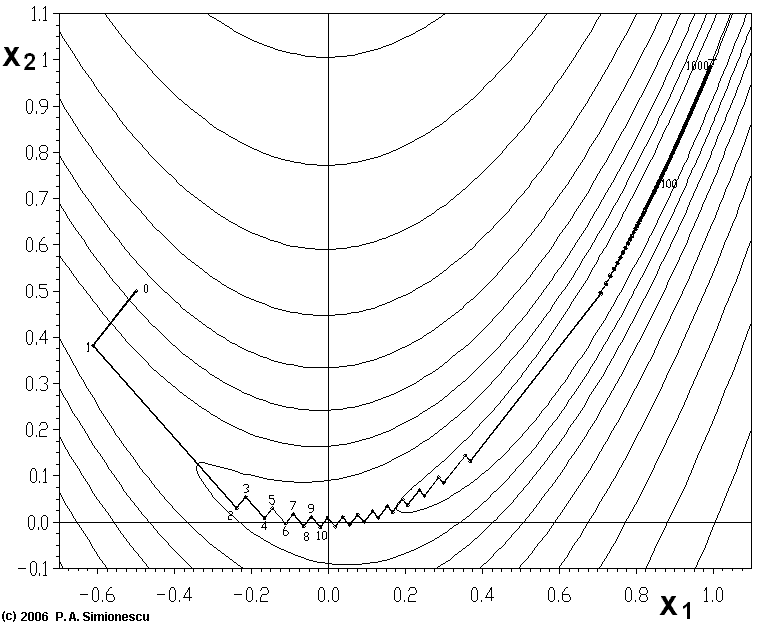
\includegraphics[width=\linewidth]{images/Banana-SteepDesc.png}
        \caption{Example of the effect of inappropriate step size, "curved valley" and flat area: slow convergence of gradient descent method. Source:~\cite{simionescu_illustration_2006}.}
        \label{fig:grad_desc_problem}
    \end{minipage}
    \hspace{0.01\linewidth}
    \begin{minipage}[t]{0.29\linewidth}
        \centering
        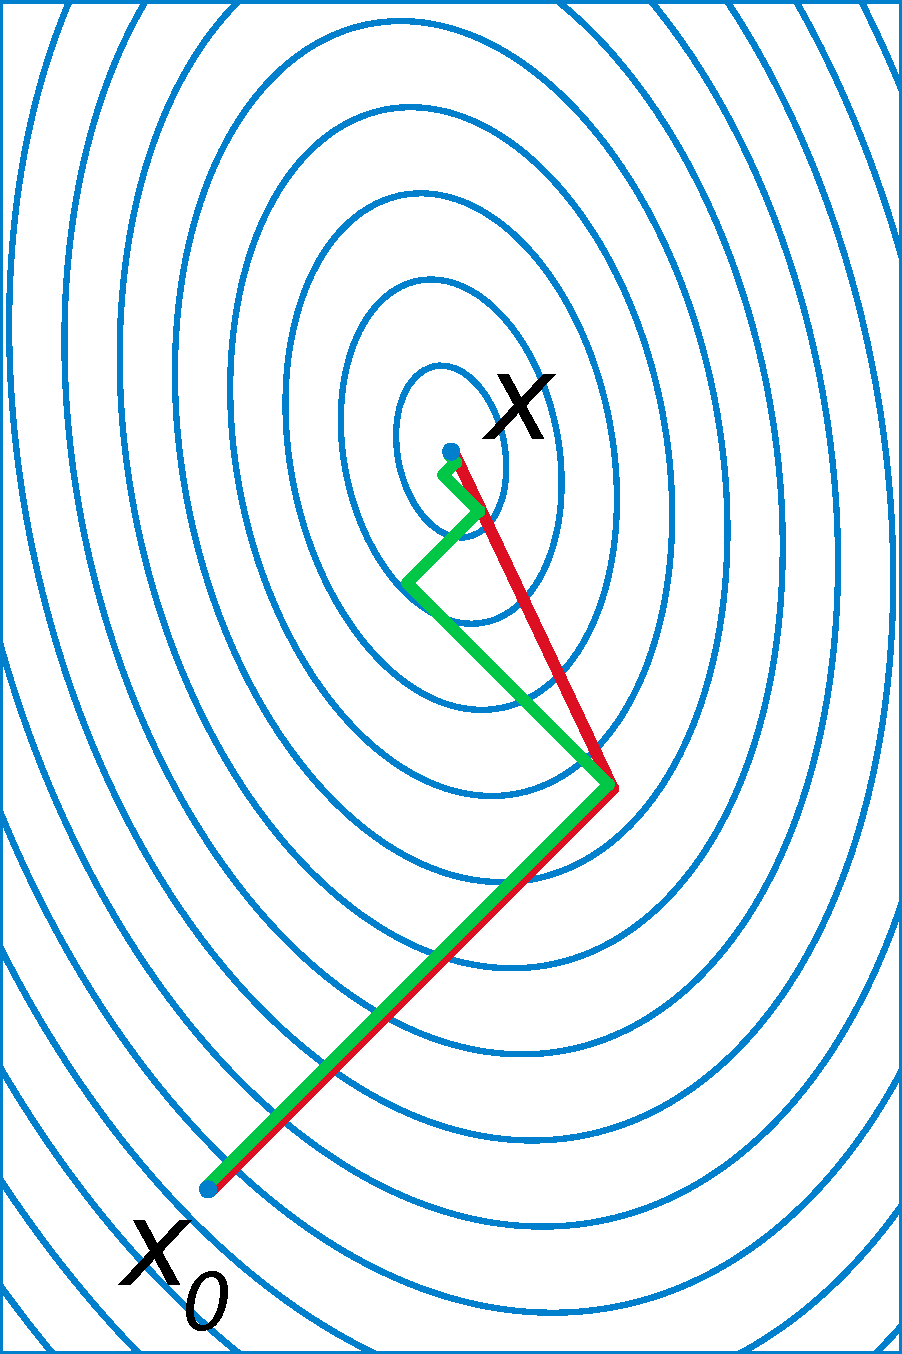
\includegraphics[width=0.45\linewidth]{images/Conjugate_gradient_illustration.pdf}
        \caption{Visualization of the advantage of the CG method compared to GD: CG requires significantly fewer steps. The green line shows the path of the GD method, red shows the path of the CG method. Source:~\cite{alexandrov_illustration_2007}.}
        \label{fig:CG_vs_GD}
    \end{minipage}
\end{figure}

The basic algorithm, but still the most popular version, can be simply summarized as follows:

\begin{algorithm}[H]
    \SetKwInOut{Inputs}{input}
    \SetKwInOut{Output}{output}
    \Inputs{vector $\mathbf{b}$ ,\\ symmetric, positive-definite matrix $\mathbf{A}$, \\ $\epsilon \in \mathbb{R}_+$ error tolerance parameter, and \\ approximate initial solution $\mathbf{x}_0$ (optional, set to $\mathbf{0}$ by default)}
    \Output{vector $\mathbf{x}$ such that $\mathbf{Ax} = \mathbf{b}$}
    \BlankLine
    Initialize $\mathbf{r}_0 = \mathbf{b} - \mathbf{Ax}_0$, $\mathbf{p}_0 = \mathbf{r}_0$, $k = 0$\\
    \While{$\norm{\mathbf{r}_k} > \epsilon$}{
        $\alpha_k = \frac{\mathbf{r}_k^* \mathbf{r}_k}{\mathbf{p}_k^* \mathbf{Ap}_k}$\\
        $\mathbf{x}_{k+1} = \mathbf{x}_k + \alpha_k \mathbf{p}_k$\\
        $\mathbf{r}_{k+1} = \mathbf{r}_k - \alpha\mathbf{Ap}_k$\\
        $\beta_k = \frac{\mathbf{r}_{k+1}^* \mathbf{r}_{k+1}}{\mathbf{r}_k^* \mathbf{r}_k}$\\
        $\mathbf{p}_{k+1} = \mathbf{r}_{k+1} + \beta_k\mathbf{p}_k$\\
        $k = k + 1$
    }
    \Return $\mathbf{x}_k$
    \caption{Conjugate Gradient (CG) method}
\end{algorithm}

It worth noting that while it is hard to find a better method for simple problems than CG, in more complex cases preconditioning is necessary to ensure fast convergence. Furthermore, there exist multiple extensions of the base CG algorithm, like the biconjugate gradient (BiCG) method and its stabilized version (BiCGSTAB)~\cite{van_der_vorst_bicgstab_1992} that removes the constraint of self-adjointness, and the non-linear versions (just to name a few: \cite{fletcher_function_1964, polak_note_1969, dai_nonlinear_1999}) that pushes even further the boundary of set of problems solvable by CG.

\subsection[Accelerated Gradient Methods]{Accelerated Gradient Methods\footnote{This section follows the presentation~\cite{kim_optimal_2017} given by Jeffrey Fessler in December, 2017.}}

Even though the conjugate gradient methods provides an effective way to accelerate the convergence, the momentum-based methods that mostly outperform them in cases of complex, non-quadratic cost functions has also a long history. First, the so called heavy ball momentum was proposed by Polyak in 1967 to accelerate convergence~\cite{polyak_methods_1964}. The resulting heavy ball iteration takes the following form:
\[\mathbf{x}_{k+1} = \mathbf{x}_k - \frac{\alpha}{L}\nabla f(\mathbf{x}_k) + \beta (\mathbf{x}_k - \mathbf{x}_{k-1})\]
where $\alpha$ and $\beta$ are simple constants, and the term $\beta (\mathbf{x}_k - \mathbf{x}_{k-1})$ is referred to as the \textit{momentum}. The names \textit{heavy ball} and \textit{momentum} comes from the physical analogy; namely, the path defined by the minimizer sequence $\{\mathbf{x}_k\}$ resembles the route of a ball rolling down from a hill. The optimal choice of $\alpha$ and $\beta$ is unfortunately not trivial. In fact, universally optimal options not exists, but there are many variants of heavy ball method with different choice of $\alpha$ and $\beta$, being optimal always only in specific use cases. Following that, Nesterov published the algorithm in 1983 that later became known as fast gradient method (FGM)~\cite{nesterov_method_1983}. In contrast to the original gradient descent scheme, it maintains two converging sequences $\{\mathbf{x}_k\}$ and $\{\mathbf{z}_k\}$, of which $\{\mathbf{x}_k\}$ is the sequence that converges to the solution. The algorithm consists of three simple steps as shown below.

\begin{algorithm}[H]
    \SetKwInOut{Input}{input}
    \SetKwInOut{Output}{output}
    \Input{convex and smooth function $f$, \\ $\epsilon \in \mathbb{R}_+$ error tolerance parameter, and approximate initial solution $\mathbf{x}_0$ (optional, set to $\mathbf{0}$ by default)}
    \Output{vector $\mathbf{x} = \argmin f(\mathbf{x})$}
    \BlankLine
    Initialize $t_0 = 1, k = 0, \mathbf{z}_0 = \mathbf{x}_0$\\
    \Repeat{$\norm{\mathbf{x}_k - \mathbf{x}_{k-1}} < \epsilon$}{
        $\mathbf{z}_{k+1} = \mathbf{x}_k - \frac{1}{L}\nabla f(\mathbf{x}_k)$\\
        $t_{k+1} = \frac{1}{2}\left(1 + \sqrt{1 + 4t_k^2}\right)$\\
        $\mathbf{x}_{k+1} = \mathbf{z}_{k+1} + \frac{t_k - 1}{t_{k+1}}(\mathbf{z}_{k+1} - \mathbf{z}_k)$\\
        $k = k+ 1$
    }
    \Return{$\mathbf{x}$}
    \caption{Fast Gradient Method (FGM)}
\end{algorithm}

Despite the seemingly different formulations, both methods use some kind of momentum rule. The main difference is that heavy ball simply performs a weighted addition of the momentum from the previous iterations and the gradient of the current position, Nesterov's method combines these term in a couterintuitive, yet optimal manner as depicted on fig.~\ref{fig:momentum}. While FGM is preferred in convex optimization problems since it is slightly faster than heavy ball method, the latter is more commonly used in the machine learning community due to its robustness in non-convex settings.

\begin{figure}[t]
    \centering
    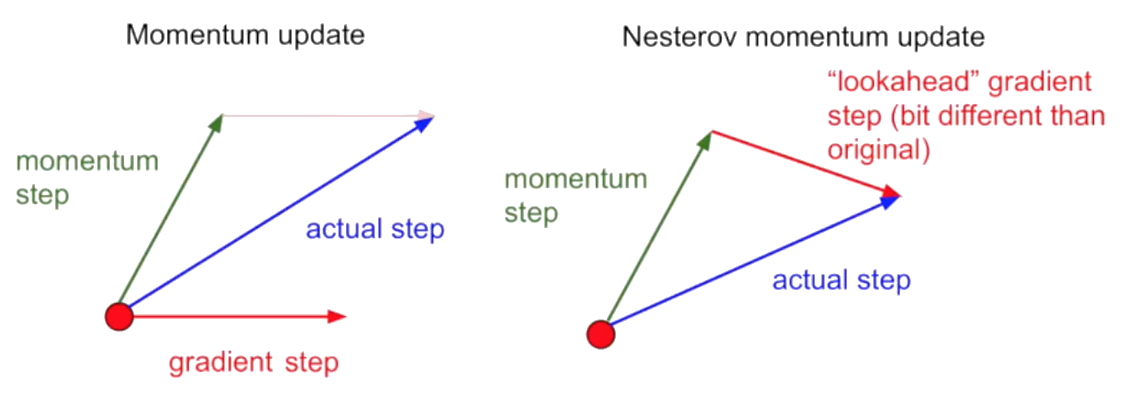
\includegraphics[width=0.8\linewidth]{images/momentum.png}
    \caption{\textbf{Difference between heavy ball momentum and Nesterov's momentum:} While the heavy ball simply performs a weighted addition of the momentum from the previous iterations and the gradient of the current position, Nesterov's method combines these term in a couterintuitive, yet optimal manner. Source: Image is adapted from~\cite{chandradevan_evolution_2017} and the idea of intuitive description of Nesterov's momentum rule as "lookahead" gradient step originates from~\cite{sutskever_importance_2013}.}
    \label{fig:momentum}
\end{figure}

Up to recent time, FGM was considered to be the fastest possible first order method for convex optimization because of its quadratic convergence proved by Nesterov. He also proved that the \textit{order} of convergence (i.e., quadratic convergence) of his algorithm is optimal indeed for first order methods. Nevertheless, the \textit{rate} of convergence of FGM is slightly sub-optimal as it was suggested by the convergence analysis performed by Drori and Teboulle in 2014~\cite{drori_performance_2014}. In their research, they considered a "meta optimization" problem, notably the minimization of worst-case convergence rate over all first order methods and all possible cost functions. As this problem is too difficult to be solved, they relaxed the problem to get a similar "meta-minimization" which can be solved by a semi-definite program. They found numerically that the relaxed bound of worst-case convergence rate for FGM is slightly below
\[\frac{2L\norm{\mathbf{x}_0 - \mathbf{x}_*}_2^2}{(N+1)^2},\]
where $N$ is the number of steps performed. Instead, they proposed a sequence of fixed step sizes calculated numerically that has approx. two times lower worst-case upper bound on convergence. Their approach, however, has a few drawbacks, such as the number of steps must be chosen in advance to ensure the improved convergence bound, and the numerical method producing these optimal step sizes is expensive both computationally and memory-wise. The next step that made this algorithm applicable in practical problems was done by Kim and Fessler in 2016, when they presented the analytical solution for the optimized step size coefficients~\cite{kim_optimized_2016} in the following form:

\begin{algorithm}[H]
    \SetKwInOut{Input}{input}
    \SetKwInOut{Output}{output}
    \Input{convex and smooth function $f$, \\ $\epsilon \in \mathbb{R}_+$ error tolerance parameter, and \\ approximate initial solution $\mathbf{x}_0$ (optional, set to $\mathbf{0}$ by default)}
    \Output{vector $\mathbf{x} = \argmin f(\mathbf{x})$}
    \BlankLine
    Initialize $\theta_0 = 1, k = 0, \mathbf{z}_0 = \mathbf{x}_0$\\
    \While{$\norm{\mathbf{x}_k - \mathbf{x}_{k-1}} > \epsilon$}{
        $\mathbf{z}_{k+1} = \mathbf{x}_k - \frac{1}{L}\nabla f(\mathbf{x}_k)$\\
        $\theta_k = \begin{cases}
            \frac{1}{2}\left(1 + \sqrt{1 + 4\theta_{k-1}^2}\right) : k = 1, 2, \ldots N - 1\\
            \frac{1}{2}\left(1 + \sqrt{1 + 8\theta_{k-1}^2}\right) : k = N
        \end{cases}$\\
        $\mathbf{x}_{k+1} = \mathbf{x}_k - \frac{1 + t_k/t_{k+1}}{L}\nabla f(\mathbf{x}_k) + \frac{t_k - 1}{t_{k+1}}(\mathbf{z}_{k+1} - \mathbf{z}_k)$\\
        $k = k + 1$
    }
    \Return{$\mathbf{x}$}
    \caption{Optimized Gradient Method 1 (OGM1)}
\end{algorithm}

This form reflects the simple modification of the existing Nesterov method that leads to the improved speed, namely the introduction of a new momentum term. The only problem is that the step size sequence still depends on the number of steps performed. Therefore, the same authors published a refined version of the algorithm~\cite{kim_convergence_2017} a year later that removes this limitation and also simplifies the implementation:

\begin{algorithm}[H]
    \SetKwInOut{Input}{input}
    \SetKwInOut{Output}{output}
    \Input{convex and smooth function $f$, \\ $\epsilon \in \mathbb{R}_+$ error tolerance parameter, and \\ approximate initial solution $\mathbf{x}_0$ (optional, set to $\mathbf{0}$ by default)}
    \Output{vector $\mathbf{x} = \argmin f(\mathbf{x})$}
    \BlankLine
    Initialize $t_0 = 1, k = 0, \mathbf{z}_0 = \mathbf{x}_0$\\
    \While{$\norm{\mathbf{x}_k - \mathbf{x}_{k-1}} < \epsilon$}{
        $\mathbf{z}_{k+1} = \mathbf{x}_k - \frac{1}{L}\nabla f(\mathbf{x}_k)$\\
        $t_{k+1} = \frac{1}{2}\left(1 + \sqrt{1 + 4t_k^2}\right)$\\
        $\mathbf{x}_{k+1} = \mathbf{x}_k - \frac{1 + t_k/t_{k+1}}{L}\nabla f(\mathbf{x}_k) + \frac{t_k - 1}{t_{k+1}}(\mathbf{z}_{k+1} - \mathbf{z}_k)$\\
        $k = k + 1$
    }
    \Return{$\mathbf{x}$}
    \caption{Optimized Gradient Method 2 (OGM2)}
\end{algorithm}

Of course, this formulation also enjoys the twice better worst-case convergence rate meaning that the new convergence bound on the helper sequence $\{\mathbf{z}_k\}$ for every iteration is
\[f(\mathbf{z}_k) - f(\mathbf{z}_*) \le \frac{1L\norm{\mathbf{x}_0 - \mathbf{x}_*}_2^2}{(k+1)^2}.\]
Moreover, Drori showed in~\cite{drori_exact_2017} that all first order algorithm have a function $f$ such that
\[\frac{L\norm{\mathbf{x}_0 - \mathbf{x}_*}_2^2}{N^2} \le f(\mathbf{z}_N) - f(\mathbf{z}_*)\]
for sufficiently large-scale problems. Thus OGM has optimal worst-case complexity, not just among the fixed step first order methods, but also among all first order methods.

\subsection{Stochastic Gradient Descent}
Sometimes the size of the problem does not allow the exact computation of even the gradient. For instance, in case of supervised learning, the problem to be solved is finding optimal parameters for a certain transform that minimizes a cost function over a huge dataset of images. Calculating the gradient of such cost function would require to load the entire dataset into the memory, but this is usually impossible as the dataset often consist millions of images requiring hundreds of gigabytes memory to load. Another example is the previously mentioned high-resolution volumentric dynamic MR image that needs \SI{256}{\gibi\byte} for a 3D image of size $512\times512\times512$ with 512 time frames assuming that each pixel is stored as a single precision complex number.

Nevertheless, the application of gradient methods to these problems are not hopeless, if the cost function can be decoupled into smaller functions. Fortunately it is very often possible. Returning to the previous examples: The cost function of the supervised learning problem is usually a sum of values of a simple function evaluated separately for each image; and the cost function of the MRI problem can often be approximated by a summation of cost values evaluated for each frame.

One possible approach is calculating the gradient for each term of the summation (this need loading only a single image/frame into the memory), and then the previously prohibiting memory demand can be reduced to an accumulating summation that needs memory allocation only for the accumulator and the current image/frame. This approach is often referred to as batch gradient descent. Another approach, called stochastic gradient descent (SGD), is applying the position update step (i.e., the step that calculates the next element of the $\{\mathbf{x}_k\}$ sequence) after the evaluation of gradient for each frame. Even though this approach uses an a less accurate approximation of the true gradient as the batch method, it appears to be surprisingly robust in many practical applications frequently giving even a better result than batch processing in highly non-convex cases. The third possibility is a combination of the first two: the dataset is divided into small partitions, and the algorithm iterates over these partitions performing the update step only after the sum of gradients within the current batch is calculated. These partitions are usually called mini-batches, and thus the name of this method is mini-batch gradient descent.

\subsection{Proximal Gradient Methods}

Besides the possibly slow convergence, the standard gradient descent method suffers from another important limitation in real-life applications; notably, the the cost function is frequently not differentiable. There are multiple ways to handle this problem, like finding a differentiable surrogate function which has minimizers near to the original problem's minimizers, or using the subgradient method~\cite{shor_minimization_2012}. While the former is particularly useful in the cases when such surrogate can be easily defined, finding a good surrogate is a very difficult problem in general. The latter, however, converges undesirably slowly in many applications. In practice, more problem-specific methods are preferred.

In image processing and machine learning applications, the so called proximal gradient methods are peculiarly popular as the underlying assumptions of these methods covers a large range of practical problems. Specifically, it only requires that the cost function $f$ to be minimized needs to be decomposable to a convex and differentiable function $g$ with Lipschitz-contiuous gradient and a general convex function $h$:
\[f(\mathbf{x}) = g(\mathbf{x}) + h(\mathbf{x}).\]
First, we can say that although $\nabla f$ does not exists, $\nabla g$ is well-defined everywhere. Second, we can define the proximal mapping
\[prox_{h,t}(\mathbf{x}) = \argmin_z \frac{1}{2t} \norm{\mathbf{x} - \mathbf{z}}_2^2 + h(\mathbf{z}).\]
This mapping basically restricts the minimization of $h$ to the \textit{proximity} of $\mathbf{x}$ by the addition of a properly scaled paraboloid around $\mathbf{x}$. Third, we can apply the forward-backward splitting scheme introduced in~\cite{martinet_breve_1970} and~\cite{bruck_weak_1977}, that is to say, we minimize $f$ by alternating the forward and backward steps where the forward step optimizes $g(x)$ via a gradient step ($\mathbf{w}_{k+1} = \mathbf{x}_k - t_k \nabla g(\mathbf{x}_k)$), and the backward step optimizes $h(\mathbf{x})$ by proximity operator ($\mathbf{x}_{k+1} = prox_{h,t_k}(\mathbf{w}_{k+1})$). That two steps can be merged into one formula:
\[\mathbf{x}_{k+1} = prox_{h,t_k}(\mathbf{x}_k - t_k \nabla g(\mathbf{x}_k)).\]

Of course, this replacement of the original optimization problem helps us only if the proximity operator can be solved easily, preferably by a closed formula. Fortunately, the $\ell_1$-norm satisfies that criterion as
\[prox_{\norm{\cdot}_1, t}(\mathbf{x}) = \Lambda_t(\mathbf{x}),\]
where $\mathcal{T}:\mathbb{R}^n \rightarrow \mathbb{R}^n$ is the so-called soft-thresholding operator defined by
\[\Lambda_t(\mathbf{x})_i = sgn(x_i) \max(|x_i| - t, 0) = \begin{cases}x_i - t & : x_i > t \\ 0 & : -t \le x_i \le t \\ x_i + t & : x_i < -t\end{cases}.\]
After this operator, the group of methods using this thresholding function are named as \textit{iterative shrinkage-thresholding algorithms} or \textit{iterative soft-thresholding alorithms} (ISTA).

In spite of the fact that it convergence only linearly, this group of methods was successfully applied to solve many non-differentiable problems, most notably the (\ref{eq:P_1}) or LASSO problem where $g(\mathbf{x}) = \norm{\mathbf{Ax - b}}_2$ and $h(\mathbf{x}) = \lambda \norm{\mathbf{x}_1}$ and the corresponding ISTA iteration is given by
\[\mathbf{x}_{k+1} = \Lambda_{\lambda t_k}(\mathbf{x}_k - t_k A^T(\mathbf{Ax}_k - \mathbf{b}))\]
as $\nabla \norm{\mathbf{Ax - b}}_2^2 = 2 \mathbf{A}^T(\mathbf{Ax} - \mathbf{b}).$ Therefore, it is easy to see the enormous significance of the contribution of a publication by Beck and Teboulle~\cite{beck_fast_2009} in which the authors showed that ISTA can be accelerated by momentum rule used in FGM leading to a slightly more complex update step defined by
\[\mathbf{x}_k = \Lambda_{\lambda t_k}(\mathbf{z}_k - 2t_k \mathbf{A}^T(\mathbf{Az}_k - \mathbf{b}))\]
\[t_{k+1} = \frac{1}{2}\left(1 + \sqrt{1 + 4t_k^2}\right)\]
\[\mathbf{z}_{k+1} = \mathbf{x}_k + \frac{t_k - 1}{t_{k+1}}(\mathbf{x}_k - \mathbf{x}_{k-1}).\]
The authors also showed that their accelerated algorithm (named Fast ISTA or FISTA) enjoys quadrati convergence. Obviously, the OGM scheme also can be extended to the proximal gradient setting, and a possible algorithm is proposed in~\cite{taylor_smooth_2017} using the update step
\begin{align*}
    & \mathbf{y}_k = \mathbf{x}_{k-1} + t A^T(\mathbf{Ax}_{k-1} - \mathbf{b})\\
    & \mathbf{z}_k = \mathbf{y}_k
        + \frac{\theta_{k-1} - 1}{\theta_k}(\mathbf{y}_k - \mathbf{y}_{k-1})
        + \frac{\theta_{k-1}}{\theta_k}(\mathbf{y}_k - \mathbf{x}_{k-1})
        + t \frac{\theta_{k-1} - 1}{\gamma_{k-1}\theta_k}(\mathbf{z}_{k-1} - \mathbf{x}_{k-1})\\
    & \mathbf{x}_k = \Lambda_{\gamma_k}(\mathbf{z}_k - 2t_k \mathbf{A}^T(\mathbf{Az}_k - \mathbf{b}))
\end{align*}
with $t = \frac{1}{L}$ where $L$ is the Lipschitz-constant of $\nabla g(\mathbf{x}) = A^T(\mathbf{Ax} - \mathbf{b})$, \[\gamma_k = \frac{1}{L}\frac{2\theta_{k-1} + \theta_k - 1}{\theta_k}, \text{ and }
\theta_k = \begin{cases}
            \frac{1}{2}\left(1 + \sqrt{1 + 4\theta_{k-1}^2}\right) : k = 1, 2, \ldots N - 1\\
            \frac{1}{2}\left(1 + \sqrt{1 + 8\theta_{k-1}^2}\right) : k = N
        \end{cases}.\]

\section{Constrained problems}

So far we discussed only problems where the cost function was expressed in a single closed formula; however, real applications very often are better characterized by an objective function that must obey some constraints on its variables as we have already seen by the formulation of the compressed sensing problem in section~\ref{section:problem formulation}. Unfortunately, a direct solution for these problems are hardly ever feasible, and therefore the most common scenario is to transform somehow these constrained problems to unconstrained ones.

A simple and intuitive way to do this transformation is using penalty methods that replaces the constrained problem with a series of unconstrained problems consisting of an addition of the cost function and the weighted sum of functions describing the constraints. In the general form, we can say that we need to find $\min f(\mathbf{x})$ subject to $c_i(\mathbf{x}) \le 0 : \forall i \in [N]$ where $N$ is the number of constraints. (Note that this formulation also contains the equality constraints as $c(\mathbf{x}) = 0$ can be replaced by two inequality constraints; i.e., $c(\mathbf{x}) \le 0$ and $-c(\mathbf{x}) \le 0$.) Penalty methods then convert this constrained formula to
\[\min f(\mathbf{x}) + \mu_k \sum_{i \in [N]} p(c_i(\mathbf{x})),\]
where $p$ is called the penalty function and $\mu_k$ are the penalty coefficients, and we solve this problem by an arbitrary solver for different $\mu_k$ values always using the solution of previous iteration as the starting point for the next iteration. Initially $\mu_k$ is chosen to be a small number, and it is increased in each iteration until it reaches infinity (or rather a sufficiently large number in practice). The intuition behind the algorithm is that first the method finds a region where the value of $f$ is small, and as the value of $\mu_k$ increases it gradually converges to a solution that satisfies the constraints (therefore the penalty function needs to map values which satisfy the constrains to a small number and give large values that violates them; e.g. $g(x) = max(0, x)^2$ and $g(x) = e^x - 1$ are both feasible options).

A similar group of methods is the class of augmented Lagrangian methods (AL) was introduced by Powell~\cite{powell_method_1969} and Hestenes in 1969 \cite{hestenes_multiplier_1969}. That class considers the problems with equality constraints specifically, that is, $\min f(\mathbf{x})$ subject to $c_i(\mathbf{x}) = 0 : \forall i \in [N]$. Compared to penalty methods, the transformed unconstrained problem contains an extra term designed to mimic a Lagrange multiplier:
\[\min f(\mathbf{x}) + \frac{\mu_k}{2} \sum_{i \in [N]} c_i(\mathbf{x})^2 + \sum_{i \in [N]} \lambda_i c_i(\mathbf{x}).\]
Similarly to penalty methods, $\mu$ coefficients are increased after each iteration, but in this case there is no need to increase them to infinity to reach the solution of the constrained problem because of the carefully weighted additional term. The "careful weighting" means that the $\lambda_i$ variables are adjusted after each iteration to give higher weight to constraints which are violated, using the update rule $\lambda_{i+1} = \lambda_i + \mu_i c_i(\mathbf{x}_i)$.

A commonly used variant of the general augmented Lagrangian scheme is the so called Alternating Direction Method of Multipliers (ADMM)~\cite{gabay_dual_1976}. This scheme works on problems in the form
\[\min_{\mathbf{x},\mathbf{z}} f(\mathbf{x}) + g(\mathbf{z}) \text{ subject to } \mathbf{Bx + Dz = c}\]
with convex functions $f$ abd $g$, matrices $\mathbf{B}$ and $\mathbf{D}$, and some vector $\mathbf{c}$. The augmented Lagrangian of this constrained problem is defined by
\[L_{\mu}(\mathbf{x, z}, \boldsymbol{\lambda}) = f(\mathbf{x}) + g(\mathbf{z}) + \boldsymbol{\lambda}^T(\mathbf{Bx + Dz - c}) + \frac{\mu}{2}\norm{\mathbf{Bx + Dz - c}}_2^2,\]
and ADMM approximates the solution of this unconstrained problem via the three steps given as
\begin{align*}
    & \mathbf{x}_{k+1} = \argmin_{x} L_{\mu}(\mathbf{x}, \mathbf{z}_k, \boldsymbol{\lambda}_k)\\
    & \mathbf{z}_{k+1} = \argmin_{z} L_{\mu}(\mathbf{x}{k+1}, \mathbf{z}, \boldsymbol{\lambda}_k)\\
    & \boldsymbol{\lambda}_{k+1} = \boldsymbol{\lambda}_k + \mu(\mathbf{Bx}_{k+1} + \mathbf{Dz}_{k+1} - \mathbf{c})
\end{align*}
For example, the LASSO problem $\min_x \norm{\mathbf{Ax - b}}_2^2 + c \norm{\mathbf{x}}_1$ takes the form
\[\min_{\mathbf{x,z}} \norm{\mathbf{Ax - b}}_2^2 + c \norm{\mathbf{z}}_1 \text{ subject to } \mathbf{x - z = 0}\]
in the ADMM framework, and its augmented Lagrangian is
\[L_{\mu}(\mathbf{x, z}, \boldsymbol{\lambda}) = \norm{\mathbf{Ax - b}}_2^2 + c \norm{\mathbf{z}}_1 + \boldsymbol{\lambda}^T(\mathbf{x + z}) + \frac{\mu}{2}\norm{\mathbf{x + z}}_2^2.\]
Finally, the ADMM steps are the following (using the previously defined soft-thresholding operator $\Lambda$):
\begin{align*}
    & \mathbf{x}_{k+1} = (\mathbf{A}^T\mathbf{A} + \mu \mathbf{I})^{-1}(\mathbf{A}^T\mathbf{b} + \mu \mathbf{z}_k - \boldsymbol{\lambda}_k)\\
    & \mathbf{z}_{k+1} = \Lambda_{c/\mu}(\mathbf{x}_{k+1} + \boldsymbol{\lambda}_k / \mu)\\
    & \boldsymbol{\lambda}_{k+1} = \boldsymbol{\lambda}_k + \mu(\mathbf{Bx}_{k+1} + \mathbf{Dz}_{k+1} - \mathbf{c})
\end{align*}.
The advantage of this scheme is that it allows distributed and parallelized computing with slight modification on the core algorithm.






\iffalse

\subsection{Majorize-Minimization Methods}

\subsubsection{Iteratively Reweighted Least Squares Algorithms}

My slideshow about first order methods: \url{https://docs.google.com/presentation/d/1tIZSSfzzHUgo9tlKlmhSUCCWD3ynzyZwnWtpBUe--6g/edit}

\subsection{Gradient Descent}
From Cauchy to recent explosion of optimization algorithm.

The nonlinear conjugate gradient method is mainly based on the same idea as gradient descent (GD) method: That method can be imagined as a hiker trying to get down from a mountain and that hiker always follows the steepest direction; i.e., he or she is moving along the negative gradient in each time step. On the other hand, while the basic GD is easy to understand, fairly efficient, and widely used method to solve unconstrained optimization problems, it has also its drawbacks compared to other variants of the method. The three main problems are 1) the optimal step size, 2) curved "valleys", and 3) flat areas on the cost function surface. 

Why would second order methods speed up convergence and why aren't we able to apply them to our problem.

\subsection{Conjugate Gradient}
How do they work, and when can conjugate gradient outperform gradient descent

\subsection{Nonlinear Conjugate Gradient Method}
Our problem, however, is nonlinear, so the CG method described above needs some further adjustment. Therefore, the nonlinear conjugate gradient (NCG) method is used to minimize the cost function $f(\mathbf{x})$, and thus reconstruct the image:
$$\mathbf{x}_{k+1} = \mathbf{x}_k + \alpha_k \mathbf{d}_k$$
\begin{align*}
    \mathbf{d}_k &=
    \begin{cases}
    -\mathbf{g}_k & k = 1 \\
    -\mathbf{g}_k + \beta_k \mathbf{d}_{k-1} & k > 1
    \end{cases},
\end{align*}
where $\mathbf{g}_k$ denotes the gradient at the $k$th step.

While that method appears to be even simpler than the CG method, unfortunately, there is no optimal way to calculate $\alpha_k$ and $\beta_k$ parameters, so multiple methods are proposed. The two main conditions of a good method are the following:
\begin{itemize}
    \item Descent property:
    \begin{itemize}
        \item Strict: Cost function must strictly decrease in each step ($\mathbf{g}_k \mathbf{d}_k < 0$)
        \item Sufficient: We can allow a certain amount of increase in cost function ($\mathbf{g}_k \mathbf{d}_k < -c ||\mathbf{g}_k||^2$)
    \end{itemize}
    \item Global convergence
    \item Fast convergence
\end{itemize}
While it is practically impossible to fully satisfy all these three conditions at the same time, but these can be used to compare the different methods.

1) To get the $\alpha_k$ parameter, the most commonly used method is line search:
$$\alpha_k = \argmin_{\alpha > 0} f(\mathbf{x}_k + \alpha_k \mathbf{d}_k).$$
Since exact line search is usually expensive and impractical, the strong Wolfe line search is often considered in the implementation of nonlinear conjugate gradient methods. It aims to find a step size satisfying the strong Wolfe conditions:
$$f(\mathbf{x}_k + \alpha_k \mathbf{d}_k) - f(\mathbf{x}_k) \leq \rho \alpha_k \mathbf{g}_k \mathbf{d}_k$$
$$|g(\mathbf{x}_k + \alpha_k \mathbf{d}_k)^T \mathbf{d}_k| \leq - \sigma \mathbf{g}_k^T \mathbf{d}_k.$$
One method to find an $\alpha$ satisfying the Wolfe conditions is backtracking line search, where the "query" point is initially moved to a certain distance from the current location along the selected direction, and then that distance is decreased in each step until the local minimum is reached.
Fig.~\ref{fig:backtracking} visualizes that method in case of a simple quadratic function.

\begin{figure}
    \centering
    \includegraphics[width=0.3\linewidth]{images/project with Wiem/backtracking.png}
    \caption{Example of backtracking line search.}
    \label{fig:backtracking}
\end{figure}

2) Similarly, to obtain the $\beta_k$, there are multiple choices. The oldest method is the Fletcher-Reeves (FR) method:
$$\beta_k^{FR} = \frac{||\mathbf{g}_k||^2}{||\mathbf{g}_{k-1}||^2}.$$
The advantage of that method that global convergence is proved for $\sigma < \frac{1}{2}$ in the Wolfe condition using inexact line search~\cite{Al-Baali}. However, the convergence is relatively slow in many cases because it may fall into some circle of tiny steps, so that method is significantly outperformed by the Polak-Ribi\`{e}re-Polyak (PRP) method:
$$\beta_k^{FR} = \frac{\mathbf{g}_k^T (\mathbf{g}_k - \mathbf{g}_{k-1}}{||\mathbf{g}_{k-1}||^2}.$$
In spite of the improved speed, that method also has a serious problem: Global convergence can only be proved for strictly quadratic functions. There exist some sophisticated line search method that ensures global convergence for all nonlinear functions, but these methods are also computationally more intensive~\cite{grippo}.
To overcome that problem, one can improve the convergence compared to FR method speed (but reduce compared to PRP) while keeping the global convergence property for Wolfe line search by combining the two methods: $\beta_k^{GN} = \max\{-\beta_k^{FR}, \min\{\beta_k^{PRP},\beta_k^{FR}\}\}.$
Although there are multiple newer methods that are more efficient, these methods fall out of the scope of that study.

3) To sum up, the algorithm used in \cite{sparse} is the following ($TolGrad$, $maxIter$, and $\mu$ variables are parameters to control the precision):
\begin{algorithm}[H]
 // Initialization:\\
 $k \leftarrow 0$; $m \leftarrow 0$; $\mathbf{g}_0 \leftarrow \nabla f(\mathbf{x}_0);  \mathbf{d}_0 \leftarrow - \mathbf{g}_0$\;
 -------------------------------------------------------------------- \\
 // Iterations:\\
 \While{$||\mathbf{g}_k\|_2 < TolGrad$ and $k > maxIter$}{
  // Backtracking line search\\
   ~~~~~~~(inner loop condition: 1st Wolfe condition)\\
  $\alpha_k \leftarrow 1$\\
  \While{$f(\mathbf{x}_k + t  \mathbf{d}_k) - f(\mathbf{x}_k) > \rho \alpha_k \cdot \mathbf{g}_k^*  \mathbf{d}_k$}{
    $\alpha_k \leftarrow \mu \cdot \alpha_k$\\
  }
 ---------------------------------------------------------------- \\
  // Changing position along the selected direction using the calculated $\alpha_k$\\
  $\mathbf{x}_{k+1} \leftarrow \mathbf{x}_{k} + \alpha_k \mathbf{d}_{k}$\\
 ---------------------------------------------------------------- \\
  // Calculate next direction\\
  $\mathbf{g}_{k+1} \leftarrow \nabla f(\mathbf{x}_{k+1})$\\
  $\gamma \leftarrow \frac{||\mathbf{g}_{k+1}||_2^2}{||\mathbf{g}_{k}||_2^2}$ // Fletcher-Reeves method\\
  $ \mathbf{d}_{k+1} \leftarrow - \mathbf{g}_{k+1} + \gamma \mathbf{x}_{k}$\\
  $k \leftarrow k + 1$\\
 }
\end{algorithm}


\subsection{Proximal Methods}
Proximal operator, Iterative Shrinkage/Soft Thresholding Algorithm, Forward-Backward Splitting with linear line search, Wolfe conditions

To solve the optimization problem that leads to image reconstruction, a simple and widely applied method is the gradient descent and its derivatives (e.g. conjugate gradient); however, they cannot be applied simply in our case because the cost function
$$f(\mathbf{x}) = \frac{1}{2} \sum_{\ell = 1}^L \sigma_\ell^{-2} \|F_\Omega \mathbf{S}_\ell \mathbf{x} - \mathbf{y}_\ell \|_2^2 + \lambda \|\mathbf{\Phi x} \|_1$$
does not have a derivative as the $\ell^1$ norm cannot be differentiated.
Finding a both universal and efficient method to solve constrained optimization problems, where either cost function or constraint does not have a gradient, is still unsolved, but we can solve that issue by restricting the class of problems to those that has the following general Lagrangian form:
$$\mathbf{\hat{x}} = \argmin_{x \in \mathcal{H}} \{E(\mathbf{x}) + R(\mathbf{x})\},$$
where $E(\mathbf{x})$ (empirical error) is continuously differentiable convex function with $\beta$-Lipschitz continuous gradient ($\|f(\mathbf{x}) - f(\mathbf{y})\| \leq \beta \|x - y\| : \forall \mathbf{x}, \mathbf{y} \in \mathbb{C}^N$), and $R(\mathbf{x})$ (regularization term) is a non-smooth, continuous function. For that class of problems, we can define the proximity operator instead of the gradient to find a local minimum in the proximity of the current location:
$$prox_f(\mathbf{v}) := \argmin_x \frac{1}{2} \|\mathbf{x} - \mathbf{v} \|_2^2 + f(\mathbf{x}).$$

\subsection{Forward-backward splitting}
One possible implementation of proximity gradient method is forward-backward splitting (FB), which consists of two consecutive steps: First, the "forward step" that optimizes $E(x)$ with gradient ($\mathbf{w}_{k+1} = \mathbf{x}_k - t_k \nabla E(\mathbf{x}_k)$), then the "backward step" optimizes $R(\mathbf{x})$ by proximity operator ($\mathbf{x}_{k+1} = prox_R(\mathbf{w}_{k+1})$). That two steps can be merged into one formula:
$$\mathbf{x}_{k+1} = prox_R(\mathbf{x}_k - t_k \nabla E(\mathbf{x}_k)).$$

\subsection{ISTA: Iterative Shrinkage-Thresholding Algorithm}
The most difficult part of FB splitting is the calculation of proximity operator in general. However, the problem can be tremendously simplified by restricting regularization term to $\ell^1$-norm, also known as LASSO (least absolute shrinkage and selection operator) regularization: $R(\mathbf{x}) = \lambda ||\mathbf{\Phi x} ||_1$. That way the proximity operator can be simplified to soft-thresholding function~\cite{combettes_wajs_2005}:
$$soft(x,c) = sign(x) \cdot max(|x| - c, 0).$$
Fig.~\ref{fig:soft-thres} shows an example for soft-thresholding functions. Because of that name, the algorithm is also commonly referred as iterative \textit{soft}-thresholding algorithm. In that special case of FB splitting, it is even possible to determine an upper bound for convergence, which is $\mathcal{O}(\frac{1}{\epsilon})$ in that case~\cite{FISTA}.

\subsection{Relaxed Forward-Backward}
While ISTA is a well-known and widely used optimization method, its convergence speed can be vastly improved by taking the "momentum" into account. As the name implies, there is an analogy from physics that explains well how that method works: Let's imagine a ball rolling down from a hill. That ball, obviously, always try to follow the gradient, but as it rolls down in one direction, it also gains speed, thus momentum and kinetic energy. If the direction gradient changes frequently, than the ball also changes directions often, and it cannot gain speed. But if there is a straight slope, then the ball gathers kinetic energy, and it takes more time to change the direction even if the direction of the gradient changes.

That phenomenon can be expressed by the momentum term, which is basically the numerical derivative of the position, and we adjust the current position by that term:
$$x_k = prox_{ \gamma || \cdot ||_1}(z_k - \frac{1}{L} \nabla E(z_k)),$$
$$z_{k+1} = x_k + \mu (x_k - x_{k-1}),$$
where $\mu$ is the weight that balances the effect of momentum and gradient. However, determining the $\mu$ value is not trivial, and the optimal value depends on the problem. Such a measurement that searches for the optimal value is presented in~\cite{peyre_2011}, and fig.~\ref{fig:mu} shows the result.

%\begin{figure}
%    \centering
%    \includegraphics[width=0.5\linewidth]{relaxed-FB.png}
%    \caption{Speed of convergence for different $\mu$ values. %Image from~\cite{peyre_2011}.}
 %   \label{fig:mu}
%\end{figure}

\subsection{FISTA: Fast Iterative Shrinkage-Thresh. Algorithm}
Whereas introducing momentum rule leads to significant gain in convergence speed, the upper bound of convergence is still $\mathcal{O}(\frac{1}{\epsilon})$, and determining an optimal $\mu$ is a problem, as well. However, Beck et al.~\cite{FISTA} presented a method that can determine $\mu$ easily in such a way that the rate of convergence is $\mathcal{O}(\frac{1}{\epsilon^2})$, which is the theoretical limit defined by Nesterov~\cite{nesterov_1983} for optimization methods:
$$x_k = prox_{ \gamma || \cdot ||_1}(z_k - \frac{1}{\beta} \nabla E(z_k)),$$
$$\tau_k = \frac{1 + \sqrt{1 + 4(\tau_{k-1})^2}}{2},$$
$$\mu_k = \frac{\tau_{k-1} - 1}{\tau_k},$$
$$z_{k+1} = x_k + \mu_k (x_k - x_{k-1}),$$
where $\beta$ can easily calculated by power iteration method (eigenvalue decomp.) because of NFFT.

The reason why that method is significantly faster than the previous method is that $\mu$ value changes through the optimization, so the effect of momentum is small in the beginning of the optimization process (as the gradient is large enough to provide good convergence speed), but later the importance of momentum is gradually increasing because the surface of cost function is flat around the solution in most cases (see fig.~\ref{fig:mu_FISTA}). That method provides even faster convergence than relaxed FB, and also solve the problem of finding optimal $\mu$ value. Fig.~\ref{fig:ISTA_vs_FISTA} shows a comparison of converge speed in case of a simple optimization problem presented in~\cite{peyre_2011}.

%\begin{figure}
 %   \centering
 %   \includegraphics[width=0.5\linewidth]{mu.png}
 %   \caption{Change of $\mu$ value during optimization steps.}
 %   \label{fig:mu_FISTA}
%\end{figure}

%\begin{figure}
 %   \centering
 %   \includegraphics[width=0.5\linewidth]{ISTA_vs_FISTA.png}
 %   \caption{Comparism of convergence speed of FB, relaxed FB, %and FISTA methods. Image from~\cite{peyre_2011}.}
 %   \label{fig:ISTA_vs_FISTA}
%\end{figure}

\subsection{FOGM: Proximal Optimized Gradient Method}
Another method to increase convergence speed is proposed in~\cite{hendrickx_2018}, which was further improved in~\cite{gueddari_2018}. The main features of that method is that it gives a changing weight ($\gamma_k$) to the proximity operator, uses a more advanced form momentum rule, and it increases $\tau$ value in the last two steps increasing the effect of momentum at the same time that helps to avoid the slowdown of the convergence in the flat area around the solution. Although these modifications do not change the theoretical lower bound for convergence speed ($\mathcal{O}(\frac{1}{\epsilon^2})$), they make the algorithm having an about two-times faster worst-case convergence speed compared to FISTA~\cite{kim, taylor}. The steps of that algorithm are the following:

\begin{algorithm}[H]
 $k \leftarrow 0$; $\tau_0 \leftarrow 1$; $\mathbf{y}_0, \mathbf{z}_0 \leftarrow$ arbitrary value\;
 \While{$k \leq K - 1$}{
  \eIf{$k < K - 1$}{
    $\tau_k \leftarrow \frac{1 + \sqrt{1 + 4(\tau_{k-1})^2}}{2}$\\
  } {
    $\tau_k \leftarrow \frac{1 + \sqrt{1 + 8(\tau_{k-1})^2}}{2}$ // Extra speed in last two steps\\
  }
  $\gamma_{k+1} \leftarrow \frac{1}{\beta} \frac{2\tau_k + \tau_{k+1}-1}{\tau_{k+1}}$ // Weight for the proximity operator\\
  $\mathbf{x}_{k+1} \leftarrow \mathbf{z}_k - \frac{1}{\beta} \nabla E(\mathbf{z}_k)$ // Move along the gradient\\
  $\mathbf{z}_{k+1} \leftarrow \mathbf{x}_{k+1} + \frac{\tau_{k} - 1}{\tau_{k+1}} (\mathbf{x}_{k+1} - x_k) + \frac{\tau_k}{\tau_{k+1}}(\mathbf{x}_{k+1} - \mathbf{y}_k) + \frac{\tau_k - 1}{\beta \gamma_k \tau_{k+1}}(\mathbf{z}_k - \mathbf{y}_k)$ // More advanced momentum rule\\
  $\mathbf{y}_{k+1} \leftarrow prox_{\gamma_{k+1}}(\mathbf{z}_{k+1})$\\
  $k \leftarrow k + 1$\\
 }
\end{algorithm}

\subsection{ADMM}
what is it and why is it good

\fi